% Plantilla TFG LaTeX LSI por:
%   Agustín Borrego <borrego@us.es>
%   Inma Hernández <inmahernandez@us.es>
% Su uso y modificación es libre.

% ̀¡Recuerda hacer copias de seguridad frecuentes durante la redacción del trabajo!
% Puedes descargar todo el código fuente del proyecto en zip en Menú > (Descargar) Fuente

\documentclass[12pt]{report}

% Paquetes LaTeX y estilos globales
\usepackage[utf8]{inputenc}
\usepackage{multicol}
\usepackage{xcolor}
\usepackage{subfigure}
\usepackage[spanish,es-tabla]{babel}
\usepackage[utf8]{inputenc}
\usepackage{graphicx}
\usepackage{titlesec}
\usepackage[bookmarks,breaklinks,colorlinks=true,allcolors=blue]{hyperref}
\usepackage{listings}
\usepackage{inconsolata}
\usepackage{float}
\usepackage{mathpazo} % Fuente Palatino
\usepackage[labelfont=bf]{caption}

\usepackage[square,numbers]{natbib}
\usepackage[nottoc,notlof,notlot]{tocbibind}  % Mete la bibliografía como capítulo en la TOC, los parámetros excluyen los otros índices de aparecer también
\usepackage{geometry}
\usepackage{amsmath}
\usepackage{parskip}
\usepackage[official]{eurosym}
\usepackage{todonotes}
\usepackage{csquotes}
\usepackage{tocbasic}  % Estilos de la TOC

% Formato del título de capítulos y secciones
\titleformat{\chapter}[block]{\normalfont\huge\bfseries}{\thechapter.}{.5em}{\Huge}[\vspace{2pt}{\titlerule[2pt]}]

\titlespacing*{\chapter}{0pt}{-19pt}{25pt}

\titleformat{\section}[block]{\normalfont\Large\bfseries}{\thesection.}{.5em}{\Large}

\titleformat{\part}[block]{\titlerule[2pt]\normalfont\Huge\bfseries\centering}{Parte \Roman{part}\\\vspace{15pt}}{0pt}{\Huge}[\vspace{2pt}{\titlerule[2pt]}]

% Tamaños y estilos de elementos en la TOC
\DeclareTOCStyleEntry[
    linefill=\bfseries\TOCLineLeaderFill,
    beforeskip=12pt,
    entrynumberformat=\chapterprefixintoc,
    entryformat=\chaptertocformat,
    pagenumberformat=\chaptertocformat,
    dynnumwidth
]{tocline}{chapter}

\DeclareTOCStyleEntry[
    % linefill=\bfseries\TOCLineLeaderFill,
    beforeskip=30pt,
    entrynumberformat=\chapterprefixintoc,
    entryformat=\parttocformat,
    pagenumberformat=\partpagetocformat,
    numwidth=0pt
]{tocline}{part}

\newcommand\chaptertocformat[1]{\large{\textbf{#1}}}%
\newcommand\chapterprefixintoc[1]{#1}%
\newcommand\parttocformat[1]{\Large{\textbf{#1}}}%
\newcommand\partpagetocformat[1]{} % Don't print the page number for parts

% Alias para estilos de texto comunes
\newcommand{\negritas}[1]{\textbf{#1}}
\newcommand{\cursiva}[1]{\textit{#1}}
\newcommand{\codigo}[1]{\texttt{#1}}

% Formato del código fuente con lstlisting
\lstset{
  basicstyle=\ttfamily,
  breaklines=true,
}

% Márgenes
\geometry{
    a4paper,
    margin=2.75cm
}
\setlength{\marginparwidth}{2cm} 

% Limite de profundidad del índice
\setcounter{tocdepth}{2}

% Eliminar el guionado
\tolerance=1
\emergencystretch=\maxdimen
\hyphenpenalty=10000
\hbadness=10000

% Indentación de párrafos
\setlength{\parindent}{.75cm}

\renewcommand{\lstlistingname}{Extracto de código}
\renewcommand*{\lstlistlistingname}{Índice de extractos de código}

% Comandos para establecer variables
\newcommand{\setTitle}[1]{\def\tfgTitle {#1}}
\newcommand{\setAuthor}[1]{\def\tfgAuthors {#1}}
\newcommand{\setDegree}[1]{\def\tfgDegree {#1}}
\newcommand{\setSupervisor}[1]{\def\tfgSupervisor {#1}}
\newcommand{\setDepartment}[1]{\def\tfgDepartment {#1}}
\newcommand{\setMonth}[1]{\def\tfgMonth {#1}}
\newcommand{\setYear}[1]{\def\tfgYear {#1}}
\newcommand{\setDedication}[1]{\def\tfgDedication {#1}}

% Estilos para el código
% Configuración genérica
\definecolor{codegreen}{rgb}{0,0.6,0}
\definecolor{codegray}{rgb}{0.5,0.5,0.5}
\definecolor{codepurple}{rgb}{0.58,0,0.82}
\definecolor{editorOcher}{rgb}{0.8, 0.3, 0} % #FF7F00 -> rgb(239, 169, 0)
\definecolor{editorGreen}{rgb}{0, 0.5, 0} % #007C00 -> rgb(0, 124, 0)

\lstdefinestyle{listingstyle}{
    backgroundcolor=\color{white},  
    keywordstyle=\bfseries\color{blue},
    numberstyle=\tiny\color{codegray},
    stringstyle=\color{editorGreen},
    commentstyle=\color{codegray},
    basicstyle=\ttfamily\color{black},
    breakatwhitespace=false,         
    breaklines=true,                 
    captionpos=b,                    
    keepspaces=true,                 
    numbers=left,                    
    numbersep=5pt,                  
    showspaces=false,                
    showstringspaces=false,
    showtabs=false,                  
    tabsize=2,
    frame=tb,
    keywords=[2]{True,False},
    literate=%
*{0}{{{\color{editorOcher}0}}}1
{1}{{{\color{editorOcher}1}}}1
{2}{{{\color{editorOcher}2}}}1
{3}{{{\color{editorOcher}3}}}1
{4}{{{\color{editorOcher}4}}}1
{5}{{{\color{editorOcher}5}}}1
{6}{{{\color{editorOcher}6}}}1
{7}{{{\color{editorOcher}7}}}1
{8}{{{\color{editorOcher}8}}}1
{9}{{{\color{editorOcher}9}}}1,
}

\lstset{style=listingstyle}
\lstset{columns=fullflexible}

\lstdefinelanguage{css}{
  keywords={color,background-image:,margin,padding,font,weight,display,position,top,left,right,bottom,list,style,border,size,white,space,min,width, transition:, transform:, transition-property, transition-duration, transition-timing-function},	
  sensitive=true,
  morecomment=[l]{//},
  morecomment=[s]{/*}{*/},
  morestring=[b]',
  morestring=[b]",
  alsoletter={:},
  alsodigit={-}
}
% JavaScript
\lstdefinelanguage{javascript}{
  morekeywords={abstract, arguments, await, boolean, break, byte, case, catch, char, class, const, continue, debugger, default, delete, do, double, else, enum, eval, export, extends, false, final, finally, float, for, function, goto, if, implements, import, in, instanceof, int, interface, let, long, native, new, null, package, private, protected, public, return, short, static, super, switch, synchronized, this, throw, throws, transient, true, try, typeof, var, void, volatile, while, with, yield},
  morecomment=[s]{/*}{*/},
  morecomment=[l]//,
  morestring=[b]",
  morestring=[b]'
}

\setlength{\parindent}{0pt}
\newcommand{\code}[1]{\texttt{\textsc{#1}}}


%%%%%%%%%%%%%%%%%%%%%%%%%%%%%%%%%%%%%%%%%%%%%%%%%%%%%%%%%%%%%%%%%%%%%%%%%%%%%%%%%%%%%

% Variables para la portada
\setTitle{Manual de instalación, despliegue y configuración de ATLAS Broadsea}

%%%%%%%% Extrayendo evidencia utilizando la herramienta ATLAS a partir de datos estandarizados según OMOP CDM


\setAuthor{Da. Maria del Valle Alonso de Caso Ortiz} % Si hay más de un autor, separarlos con \\
\setDegree{Grado en Ingeniería de la Salud} % Cambiar si es necesario
\setSupervisor{Da. Silvia Rodríguez Mejías \\ Dr. Carlos Parra Calderón} % Si hay más de un tutor, separarlos con \\
\setDepartment{Innovación Tecnológica \\ Hospital Universitario Virgen del Rocío}
\setMonth{junio} % Dejar sólo el mes de la convocatoria en que se presenta el trabajo
\setYear{2023/24} % Por ejemplo, 2022/23

%%%%%%%%%%%%%%%%%%%%%%%%%%%%%%%%%%%%%%%%%%%%%%%%%%%%%%%%%%%%%%%%%%%%%%%%%%%%%%%%%%%%%

% Dedicatoria del trabajo
% Si no se desea incluir, comentar o borrar la línea siguiente para eliminar la página de dedicatoria
%\setDedication{A mi padre y a mi madre, por inculcarme la pasión por el estudio y acompañarme incondicionalmente en cada etapa del camino.}

%%%%%%%%%%%%%%%%%%%%%%%%%%%%%%%%%%%%%%%%%%%%%%%%%%%%%%%%%%%%%%%%%%%%%%%%%%%%%%%%%%%%%

% Comienzo del documento
\begin{document}

    % Portada y secciones no numeradas
    \thispagestyle{empty} % Impide que se incluya número de página en la portada
\begin{center}

\vspace*{1cm}


\includegraphics[width=\textwidth]{figures/etsii_us.png}

\vspace*{2.5cm}
\begin{large}
TRABAJO FIN DE GRADO
\end{large}

\vspace*{0.1in}
\textbf{\huge \tfgTitle}

\vspace*{.5in}

{\large Realizado por}\\
\textbf{\Large \tfgAuthors}

\vspace*{2cm}

\textbf{Para la obtención del título de}\\
{\large \tfgDegree}

\vspace*{0.2in}

\textbf{Dirigido por}\\
{\large \tfgSupervisor}\\

\vspace*{0.2in}

\textbf{En el departamento de}\\
{\large \tfgDepartment}

\vspace*{.6in}
\textbf{\Large Convocatoria de \tfgMonth, curso \tfgYear}

\end{center}

% Dedicatoria
\ifdefined\tfgDedication
    \newpage
    \thispagestyle{empty}
    
    \vspace*{\fill}
    \begin{center}
    \textit{\tfgDedication}
    \end{center}
    \vspace*{\fill}
\fi

\clearpage\setcounter{page}{1} % Comienza a incluir números de página a partir de aquí
\pagenumbering{roman} % En números romanos
   
    % Índice del documento y de figuras
    \begingroup
        % Los enlaces son normalmente azules, pero en los índices se configuran a negro para que no aparezca todo azul
        \hypersetup{linkcolor=black}
        \tableofcontents
        %\listoffigures
        %\listoftables
        %\lstlistoflistings
    \endgroup
    
    % Cambia el estilo de números de página de romanos a normal
    \clearpage\pagenumbering{arabic}
    
    % Capítulos del trabajo
    \chapter{Introducción, Contexto y Motivación}\label{cap:introduccion}

%Este apartado tiene un tono un poco más personal,
%al fin y al cabo relata mi vivencia y opinión subjetiva sobre el TFG

\section{Introducción}

En palabras de Malcom X, \textit{"la educación es el pasaporte hacia el futuro, ya que el mañana pertenece a aquellos que se preparan para el hoy"}, y tanto es así que han sido cuatro años de preparación y dedicación día a día los que me han ido formando personal y académicamente hasta alcanzar la realización de este Trabajo de Fin de Grado, que abre las puertas de mi futuro profesional.

%%MODIFICACIÓN--------------------------------------
En esta primera sección se presenta el contexto y la motivación que trascienden a la realización del Trabajo.
%%MODIFICACIÓN-------------------------------------------


\section{Contexto // por el que se selecciona este topico //}



%Los tiempos que corren ahora son tiempos cambiantes, Industria 4.0, el auge de las IA, la importancia de la interoprerabilidad y los estándares... 

%- Propuestas a nivel europeo? OHDSI?


%- Hablar de OHDSI EN SEVILLA

%    [Innodata2023]
    
%- La selección de este tópico se debe al creciente interés por el estándar de OHDSI en Sevilla (Hospital Macarena y/o Hospital V del Rocio) y en España.

%- Comentar Aplicaciones reales y actuales del estandar. Además del interés a nivel mundial (Ohdsi en Europa Y en america del norte). Ohdsi community.
    


\section{Motivación}

%Mi motivación personal de entrar en el mundo del %análisis de datos clínicos utilizando  esta %herramienta prometedora..






    







    \chapter{Despliegue por defecto.} \label{cap:02Despliegue}

El despliegue de ATLAS en Docker es muy sencillo y está muy bien documentado en su repositorio de github  \cite{githubBroadsea}.  Igualmente, en este manual se detallan nuevamente los pasos para la configuración y despliegue de la herramienta, añadiendo algunos pasos relevantes adicionales.

\section{Requisitos para el despliegue} \label{sec:02requisitos}

\begin{enumerate}
    \item Descargar e instalar Docker. Lo más sencillo es seguir las instrucciones de la \href{https://docs.docker.com/engine/install/}{página web oficial} para la descarga y seguir la configuración por defecto para la instalación.
    
    \item Descargar e instalar Git. Lo más sencillo es seguir las instrucciones de la \href{https://git-scm.com/downloads}{página web oficial} para la descarga y seguir la configuración por defecto para la instalación.
\end{enumerate}

\section{Deployment} \label{sec:02Deployment}

En este primer despliegue rápido de ATLAS, se desplegarán las configuraciones por defecto de la herramienta, siguiendo la guía de implementación rápida \textit{(Quick Start)} del mismo repositorio de github.

\begin{enumerate}
    \item Por tanto, el primer paso para desplegar ATLAS es clonar localmente el repositorio de github de Broadsea. Una forma rápida de hacerlo es copiar la siguiente línea de código en el \code{cdm}.

\begin{lstlisting}[language=sh]
        git clone https://github.com/OHDSI/Broadsea.git
\end{lstlisting}

    \item El segundo paso, es desplegar el contenedor docker. Para ello, situar el puntero del \code{cdm}, en la carpeta donde se ha copiado el repositorio de github de Broadsea.

\begin{lstlisting}[language=sh]
        cd ruta\del\repositorio\Broadsea\local
\end{lstlisting}

    Una vez situado en la carpeta raíz del repositorio, se jecuta el comando que instalará y desplegará el perfil por defecto del contenedor docker en la máquina local.

\begin{lstlisting}[language=sh]
    docker compose pull && docker-compose --profile default up -d
\end{lstlisting}

\end{enumerate}

\section{Comprobación de despliegue correcto} \label{sec:02comprobacion} 

Se puede comprobar que se ha instalado correctamente el contenedor de Broadsea en la máquina local de distintas formas, tal y como se presenta a continuación.

\begin{enumerate}[label=\alph*]

    \item \textbf{Comprobación a través de Docker Desktop.} La forma más sencilla de interactuar con el contenedor de Broadsea es a través de Docker Desktop. Ejecutando dicho programa, en la sección \textit{''containers"} se muestran todos los contenedores que están corriendo en el equipo. En este caso, debe aparecer un multi-contenedor llamado "broadsea" que contenga seis contenedores, tal y como se muestra en la Figura \ref{fig:dockerDesktop} ''Captura de pantalla del contenedor Broadsea en Docker Desktop''.
    
\begin{figure}[H]
    \centering
    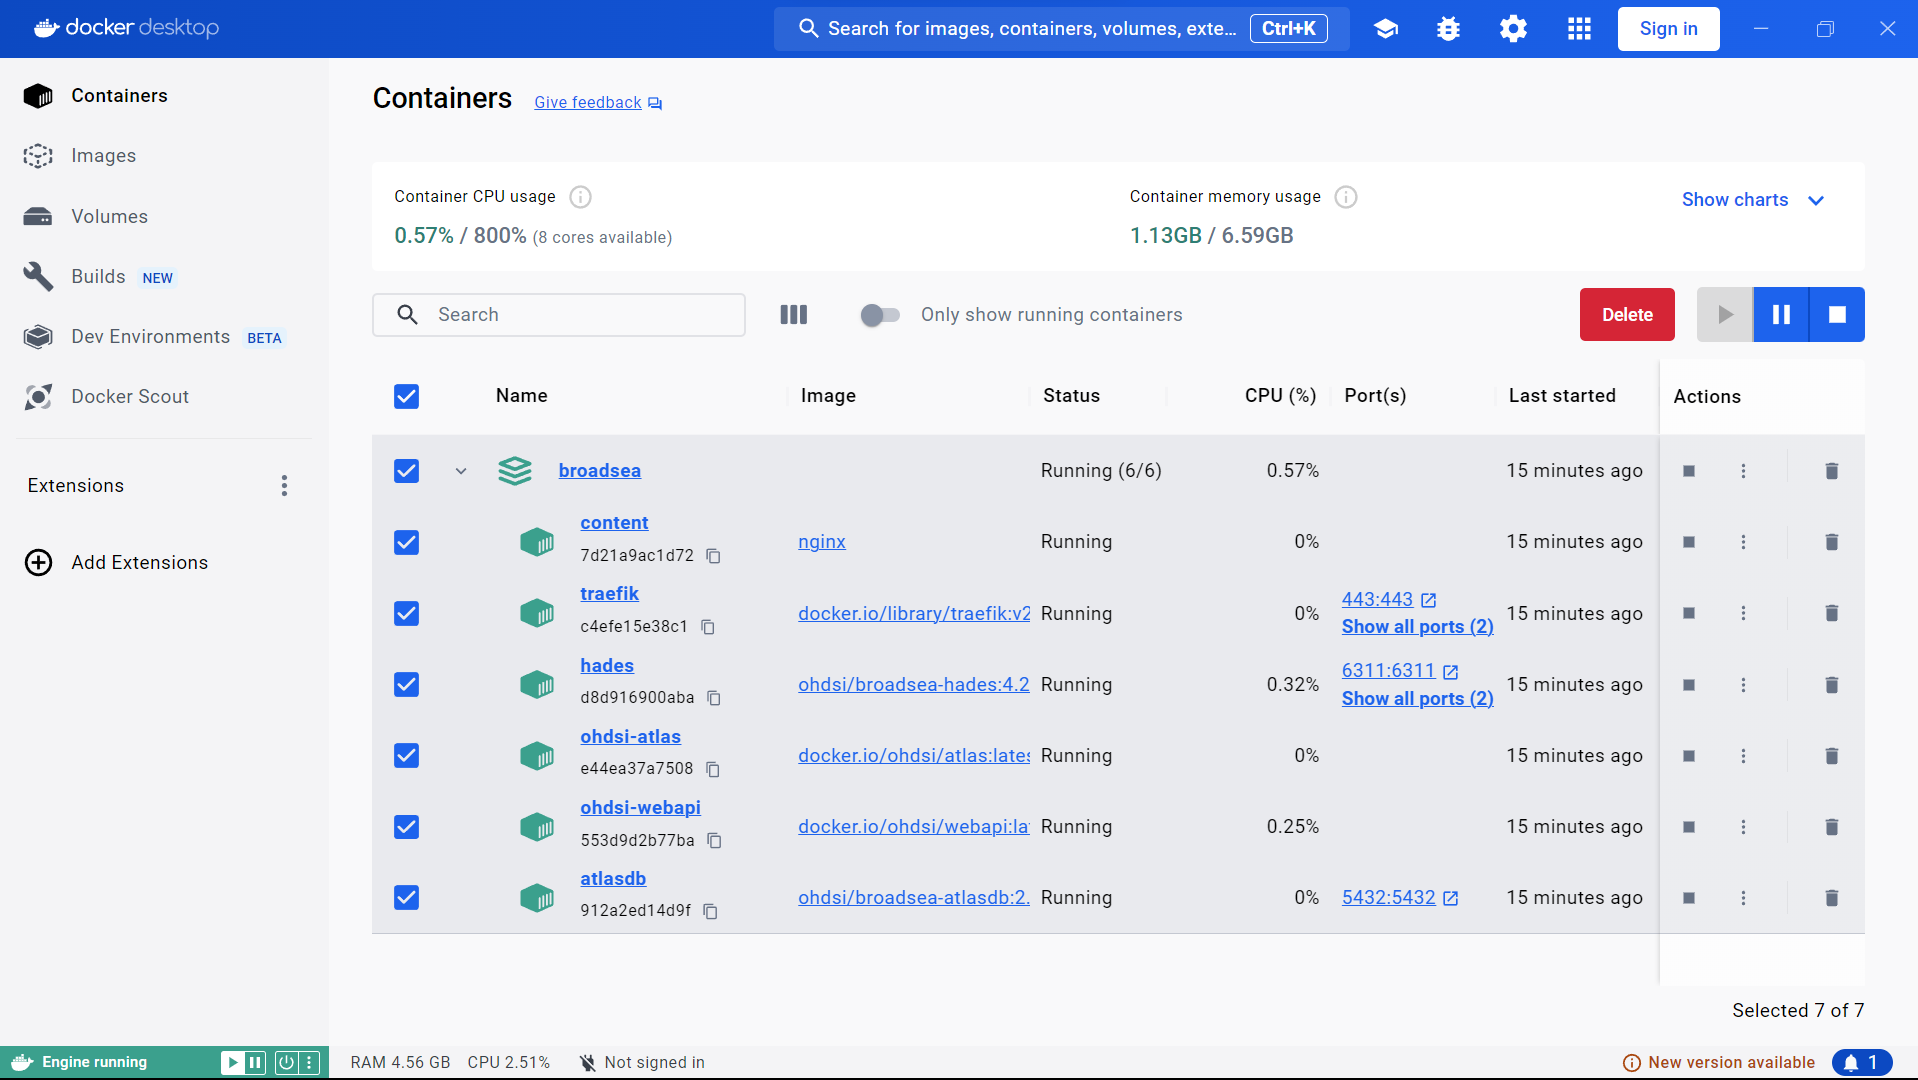
\includegraphics[width=0.90\textwidth]{figures/dockerDesktop.png}
    \caption{Captura de pantalla del contenedor Broadsea en Docker Desktop}
    \label{fig:dockerDesktop}
\end{figure}

    Mediante el panel de control de Docker se puede iniciar, pausar o detener cada contenedor (o todos a la vez) fácilmente y en cualquier momento. Por esto se dice que Broadsea ofrece servicios \textit{a-la-carte}.

    \item \textbf{Comprobación a través del \code{cmd}.} Otra forma de interactuar con el contenedor Docker es a través del \code{cmd}, ejecutando el comando \code{docker ps}, que muestra un listado de todos los contenedores que está ejecutando la máquina local. Con esta estrategia deberían mostrarse igualmente los mismos seis contenedores pertenecientes a broadsea, tal y como se muestra en la Figura \ref{fig:dockerCMD} ''Captura de pantalla del comando \code{docker ps } en el \code{cmd}''

\begin{figure}[H]
    \centering
    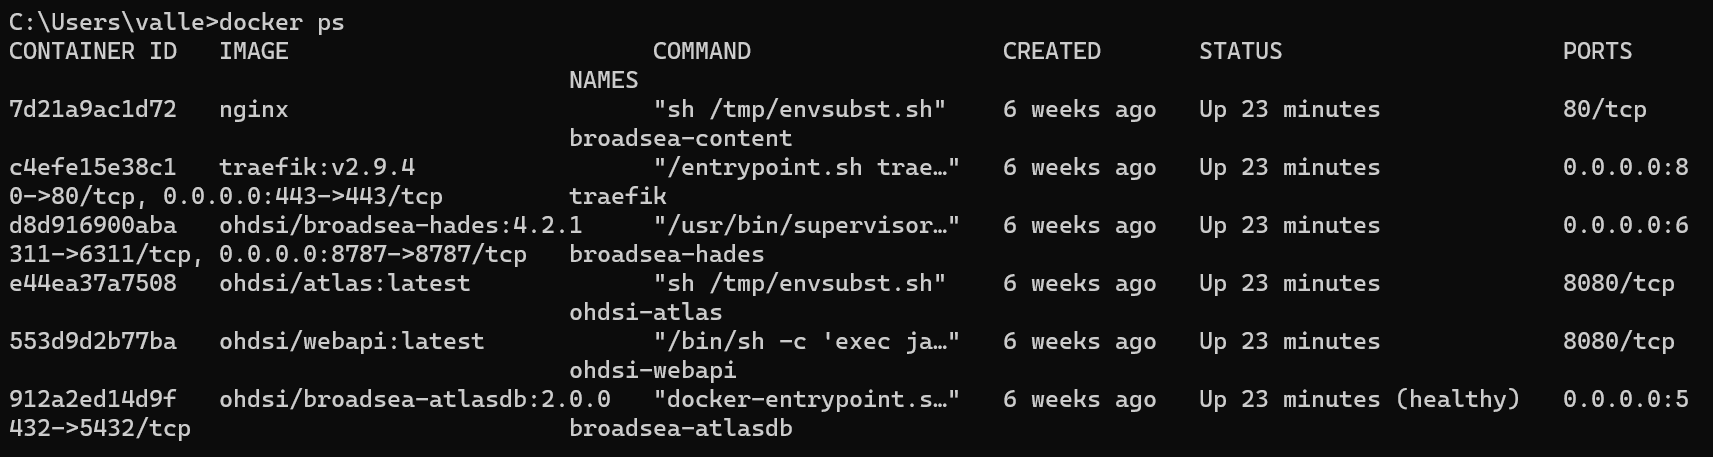
\includegraphics[width=0.90\textwidth]{figures/dockerCMD.png}
    \caption{Captura de pantalla del comando \code{docker ps } en el \code{cmd}}
    \label{fig:dockerCMD}
\end{figure}
    
    \item \textbf{Comrpobación a través del navegador.} Por último, para acceder a los servicios de Broadsea hay que abrir en el navegador web (Chrome recomendado) el servidor en el que se alojan los servicios. Por defecto, Broadsea se aloja en el servidor 127.0.0.1 (véase \ref{sec:01Postgre}).  Por tanto, introducir la dirección en el navegador para explorar las herramientas del contenedor, tal y como se muestra en la Figura \ref{fig:broadseaCap} ''Captura de pantalla del servidor Broadsea ejecutado en Chrome''.

    \begin{figure}[H]
    \centering
    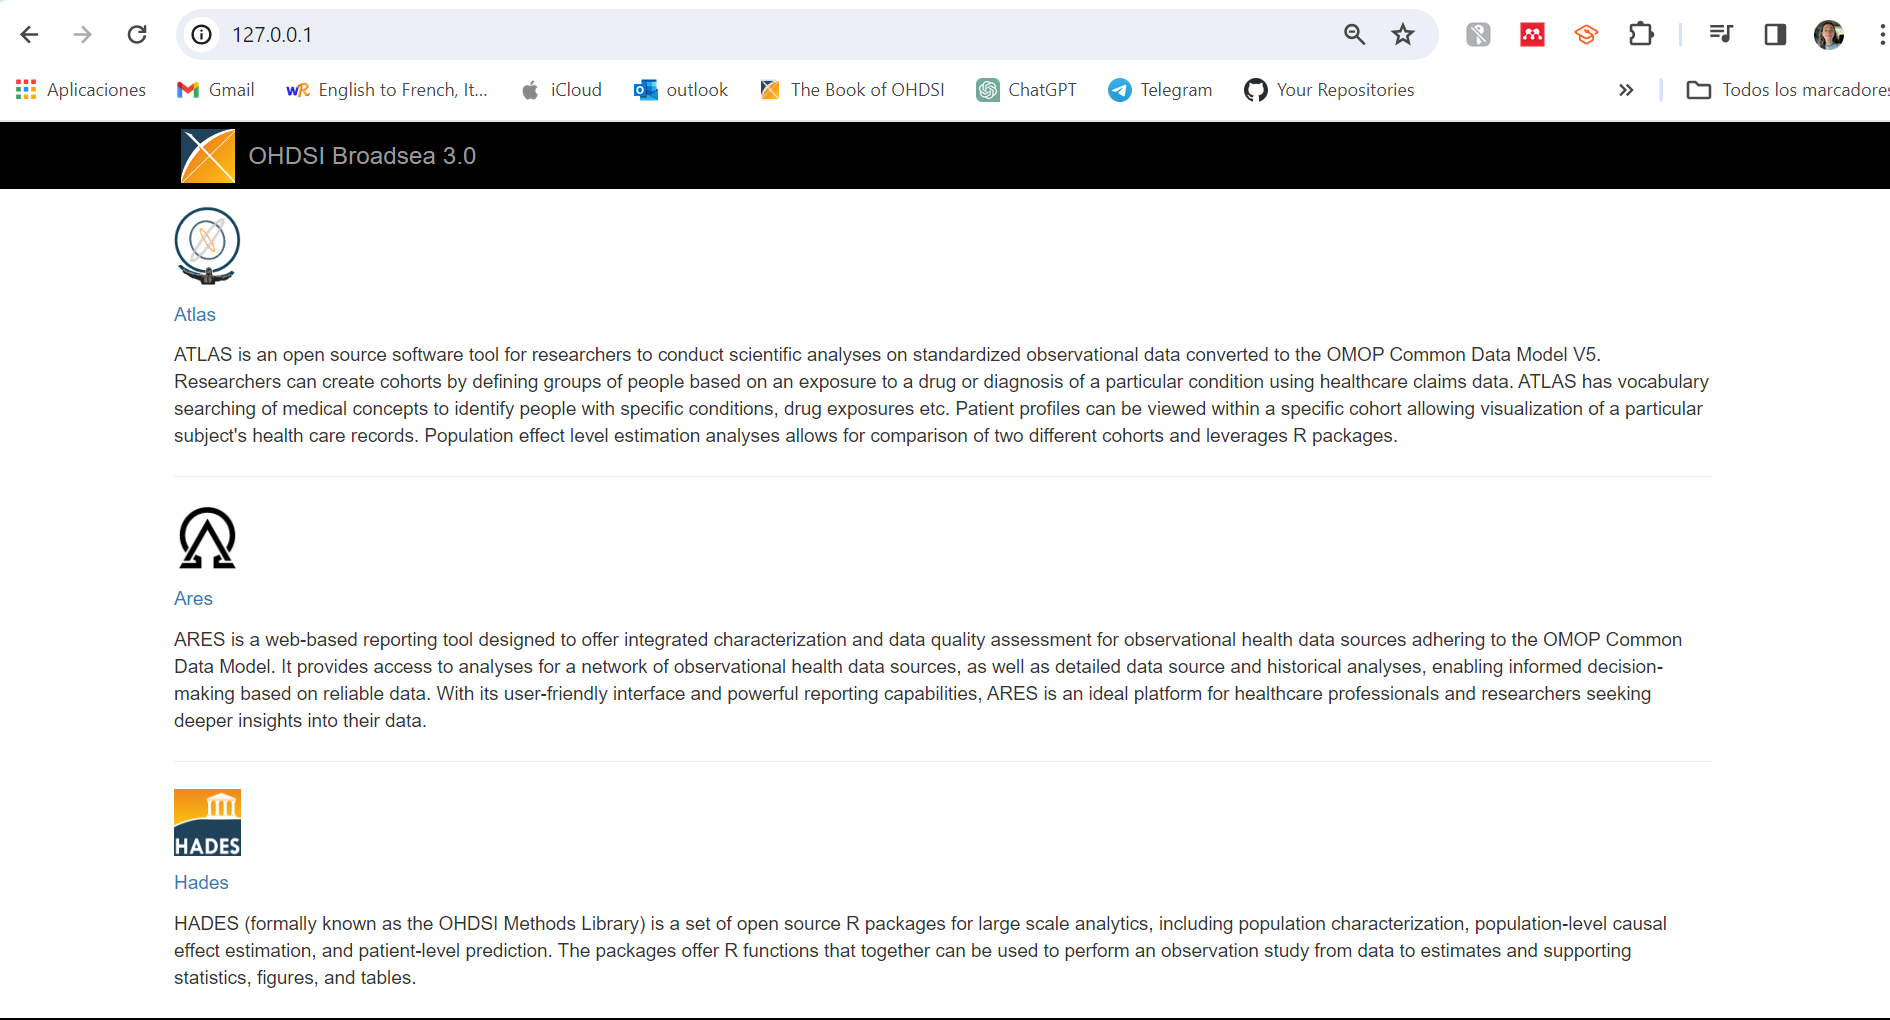
\includegraphics[width=0.90\textwidth]{figures/broadseaCap.png}
     \caption{Captura de pantalla del servidor Broadsea ejecutado en Chrome}
    \label{fig:broadseaCap}
\end{figure}
    
    Se puede comprobar o modificar el servidor exacto dónde se aloja el contenedor revisando el parámetro \code{BROADSEA\_HOST} de la sección 1 del archivo \code{.env} (para mayor información véase \ref{sec:01Docker} ''Entorno Docker de Broadsea'') de la ruta local del repositorio clonado . 

\begin{figure}[H]
    \centering
    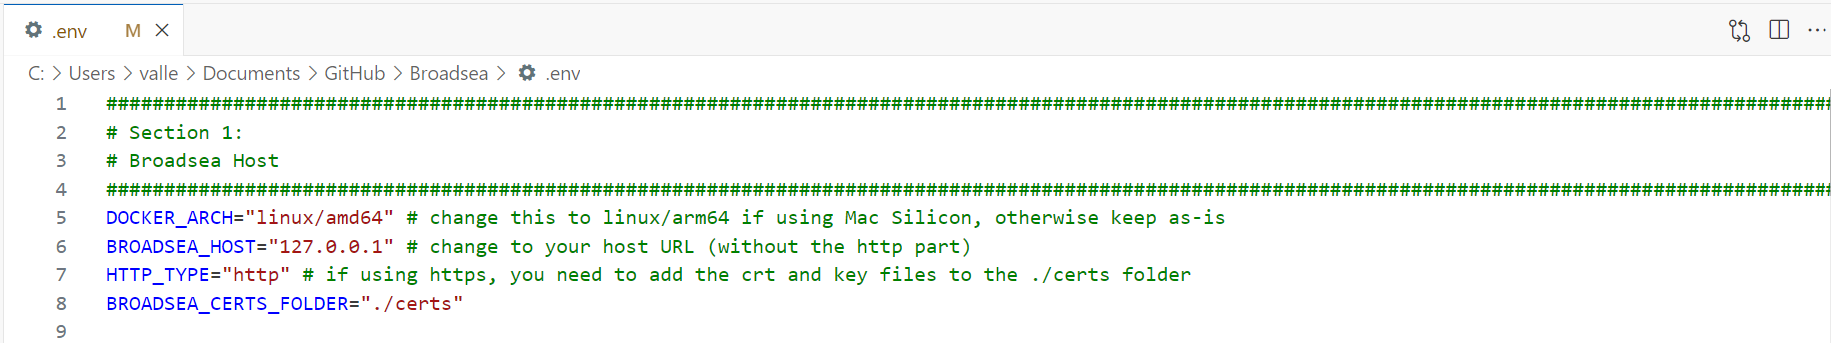
\includegraphics[width=0.90\textwidth]{figures/seccion1env.png}
    \caption{Captura de pantalla de la sección 1 del archivo \code{.env}.}
    \label{fig:seccion1env}    
\end{figure}

    En esta guía de implementación, no se va a modificar la dirección del servidor para la configuración de Broadsea, para no desconfigurar el entorno por defecto de la herramienta. Por tanto, el servidor de Broadsea durante todo el transcurso del manual será \code{127.0.0.1}, tal y como se recomienda en \cite{githubBroadseaDB} y como se muestra en la Figura \ref{fig:broadseaCap} ''Captura de pantalla del servidor Broadsea ejecutado en Chrome''

\end{enumerate}

    %Es interesante notar que Broadsea permite el acceso interactivo a la herramienta Atlas, que es la que nos interesa en este caso, pero también a Ares y a Hades, otras dos herramientas muy relacionadas (véase \ref{sec:01descripBroadsea} ''Descripción de Broadsea'').

    La ejecución de ATLAS en Broadsea es similar a ATLAS demo \cite{atlasDEMO}, aunque con algunas diferencias. En primer lugar, Broadsea solo ejecuta, por defecto, una base de datos, que es la base de datos de Eunomia (véase \ref{sec:01Postgre} ''Entorno PostgreSQL de Broadsea'').

\begin{figure}[H]
    \centering
    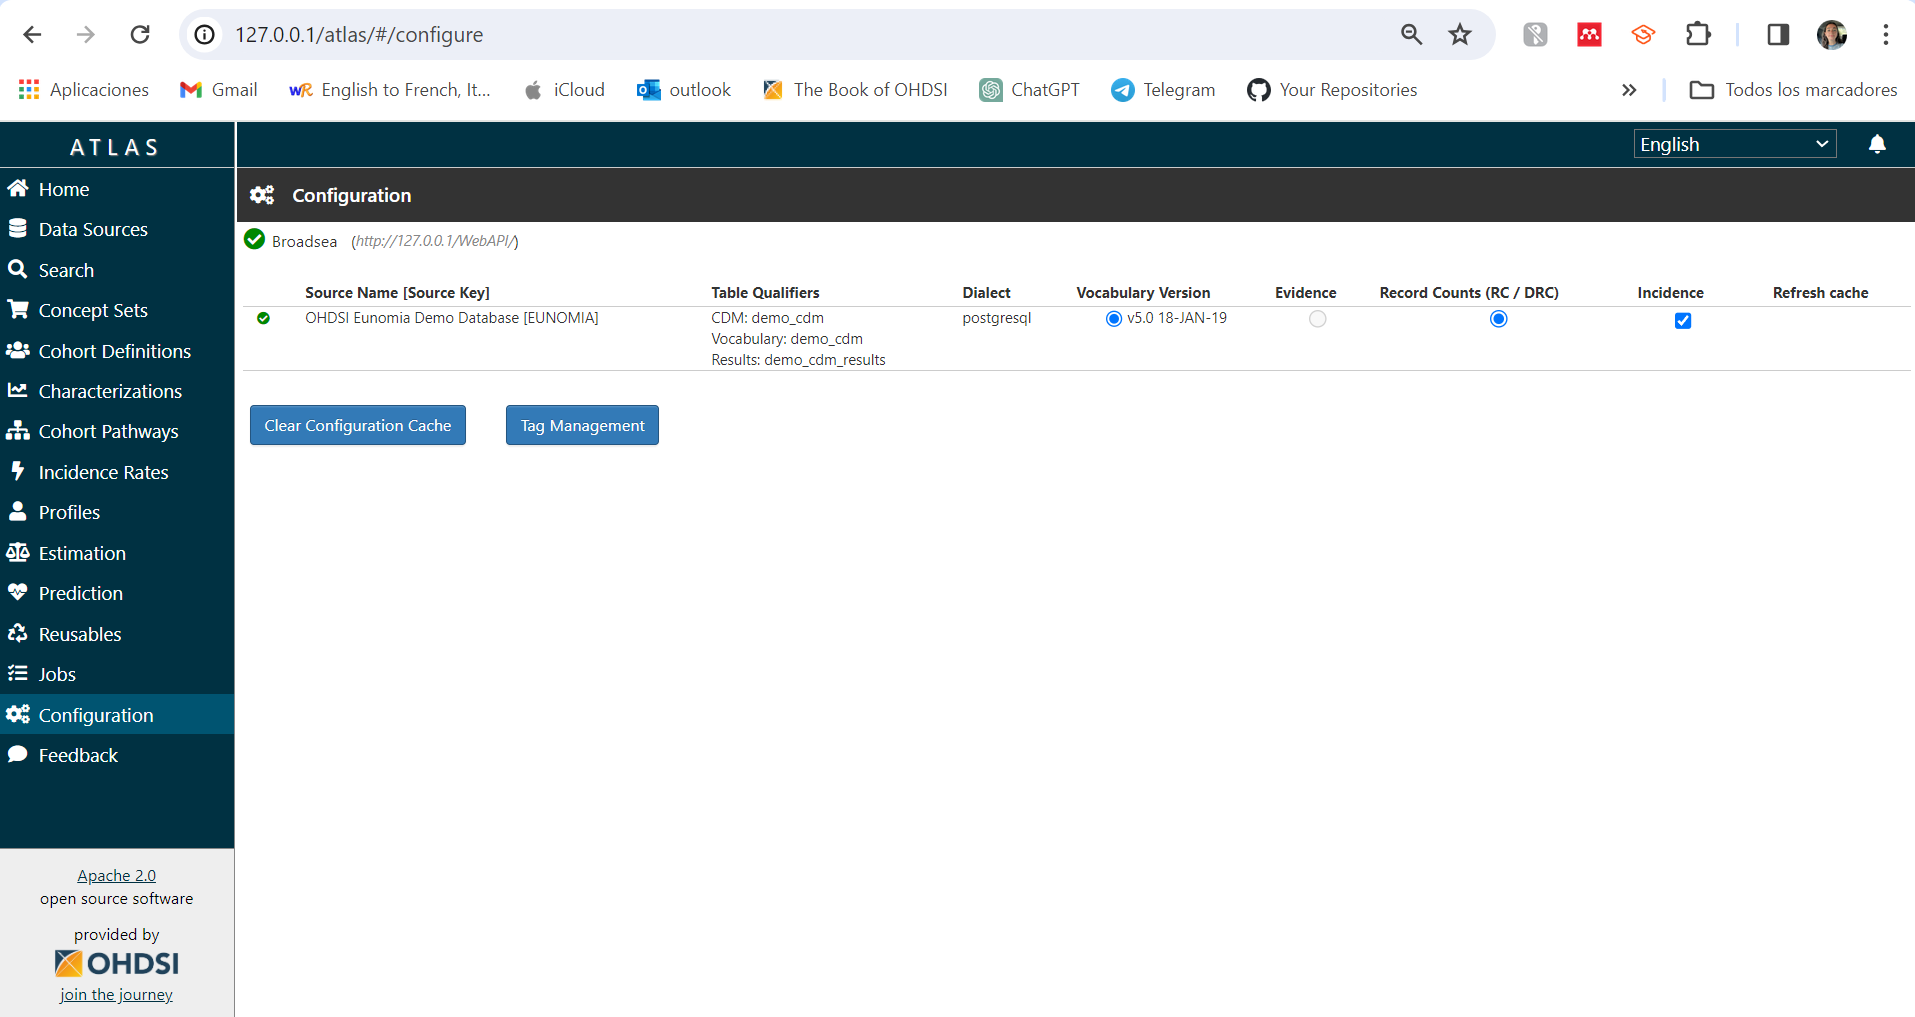
\includegraphics[width=0.90\textwidth]{figures/atlasBroadseaDB.png}
     \caption{Captura de pantalla de base de datos que utiliza ATLAS Broadsea}
    \label{fig:atlasBroadseaDB}
\end{figure}

    Por otra parte, y en contraste con la versión demo, ya no aparecen las entradas y estructuras que generan otros usuarios. La herramienta se presenta vacía, para ser completada solo con la información que el usuario local introduzca.

\begin{figure}[H]
    \centering
    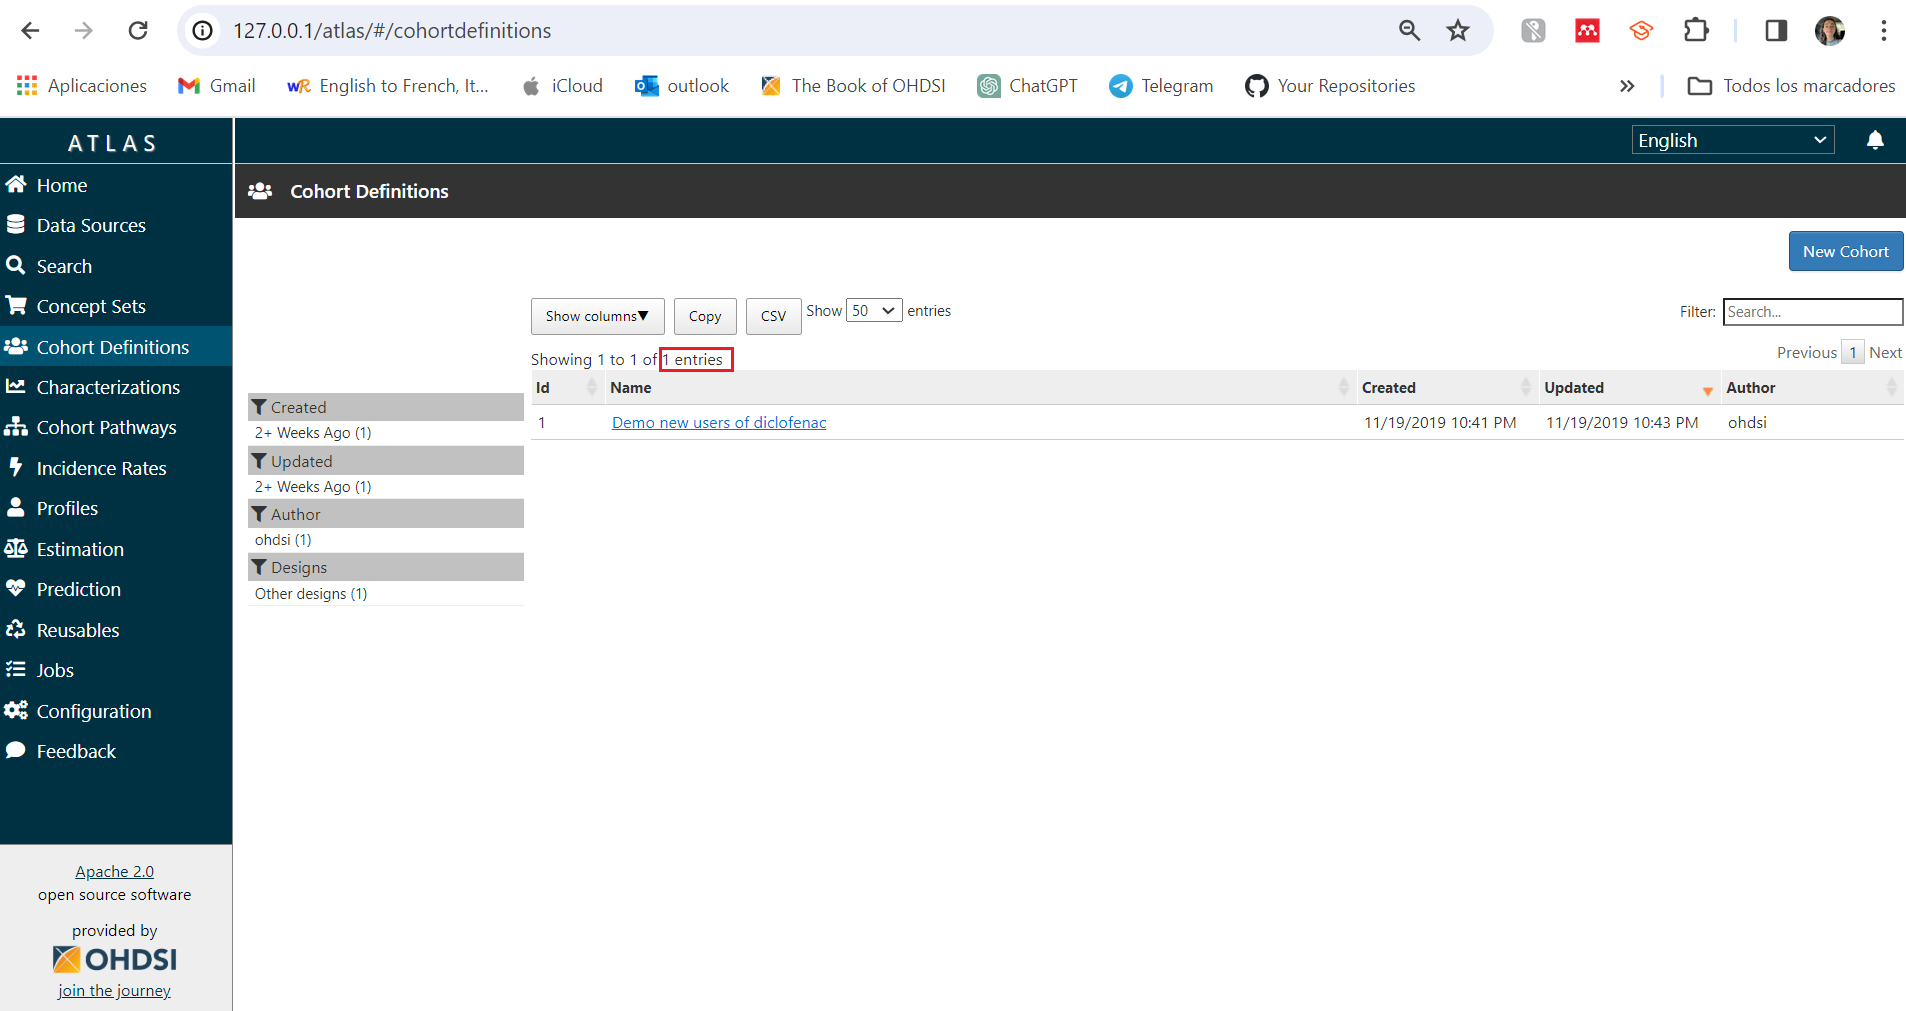
\includegraphics[width=0.90\textwidth]{figures/atlasBroadseaCD.png}
     \caption{Captura de pantalla señalando el número de entradas de definición de cohorte que almacena ATLAS Broadsea}
    \label{fig:atlasBroadseaCD}
\end{figure}
    

\section{Solución de posibles errores}

\subsubsection{Error: No se puede acceder a este sitio web. La página 127.0.0.1 ha rechazado la conexión.}

Problema: Al introducir el servidor de Broadsea en el buscador del navegador aparece esta págian de error que impide conectar con el entorno.

\begin{figure}[H]
    \centering
    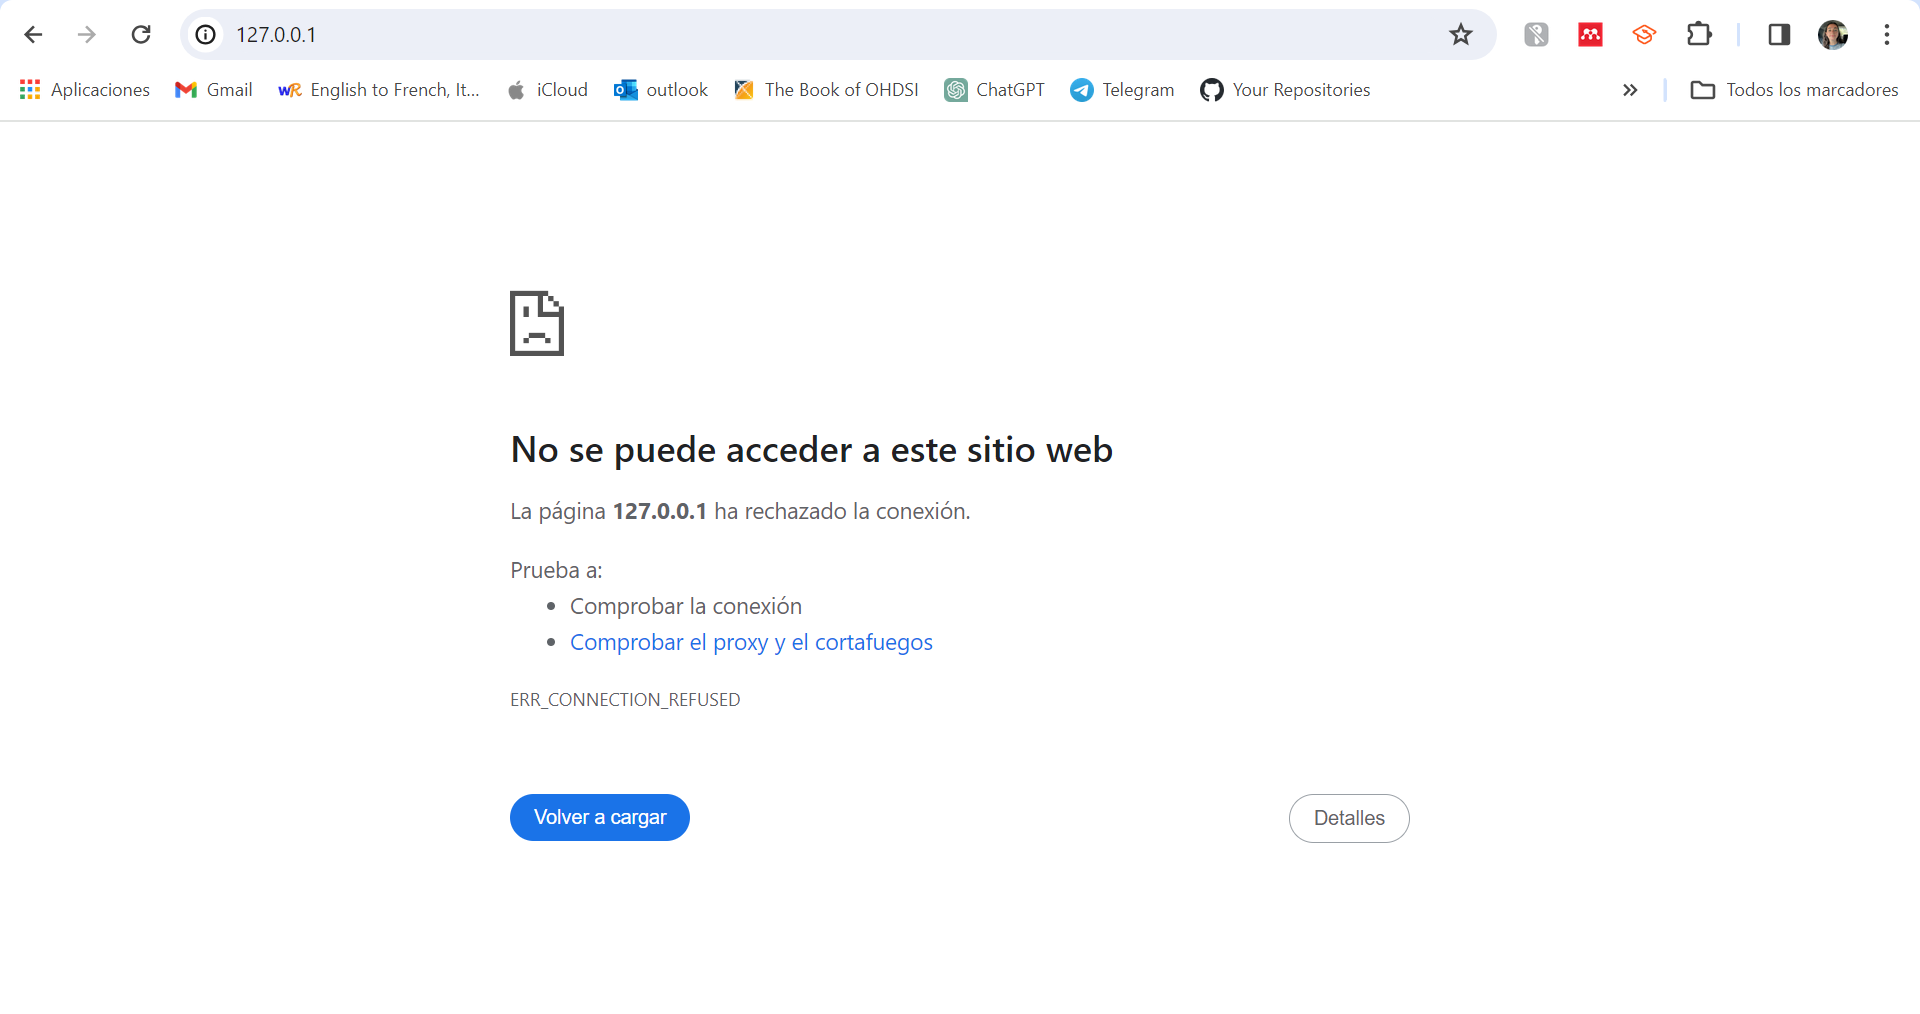
\includegraphics[width=0.90\textwidth]{figures/Error02NoSePuede.png}
     \caption{Captura de pantalla del error}
    \label{fig:Error02NoSePuede}
\end{figure}

Motivo: No se puede acceder al entorno Broadsea porque los contenedores Docker están detenidos.

Solución: Comprobar que todos los contenedores de docker implicados están corriendo. Para ello acceder a Docker Desktop y ejecutar todos los contenedores del multicontenedor de Broadsea. Una vez ejecutados todos los contenedores, si el problema persiste recargar varias veces la página.

\subsubsection{Error: Application initialization failed. Unable to connect to an instance of the WebAPI. Please contact your administrator to resolve this issue.}

Problema: Al abrir la herramienta ATLAS Broadsea aparece en rojo este error que impide conectar con la herramienta.

\begin{figure}[H]
    \centering
    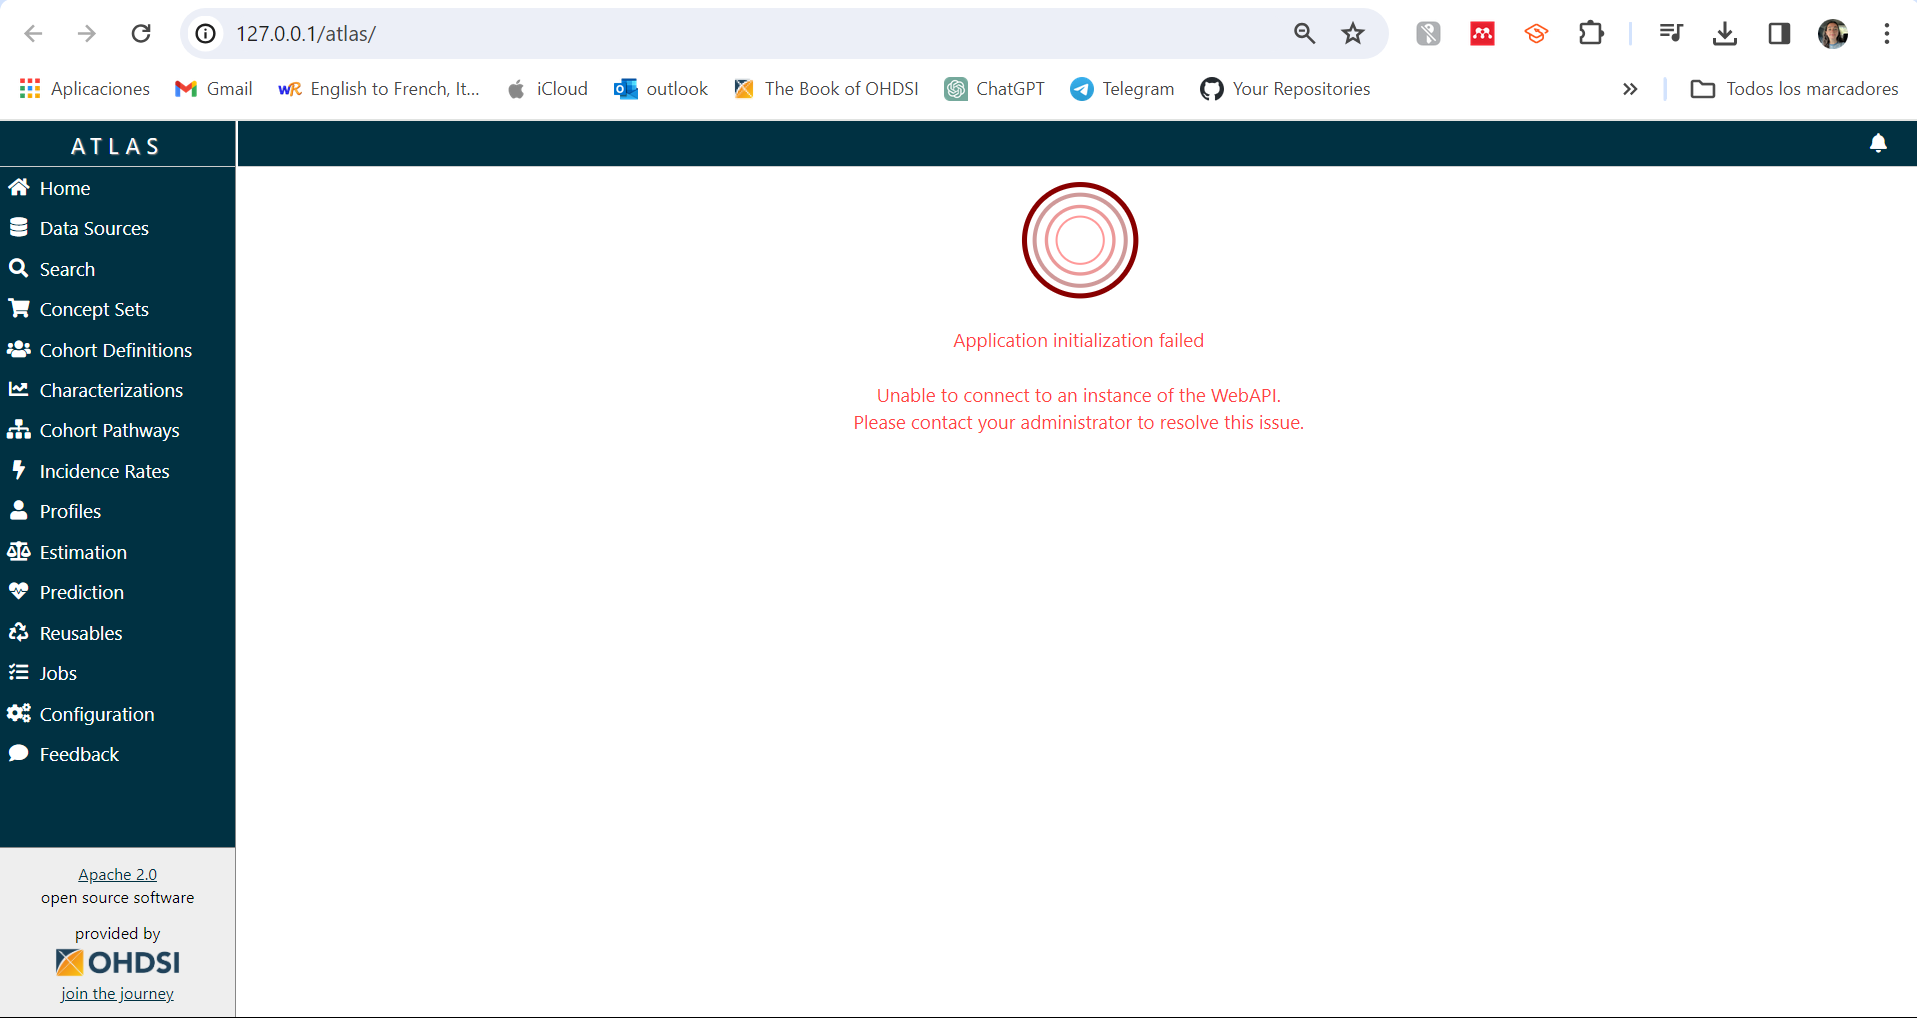
\includegraphics[width=0.90\textwidth]{figures/Error02AppFailed.png}
     \caption{Captura de pantalla del error}
    \label{fig:Error02AppFailed}
\end{figure}

Motivo: La aplicación falla al inicializarse porque no se está ejecutando correctamente el entorno docker de Broadsea.

Solución: Comprobar que todos los contenedores de docker implicados están corriendo. Para ello acceder a Docker Desktop y ejecutar todos los contenedores del multicontenedor de Broadsea. Una vez ejecutados todos los contenedores, si el problema persiste recargar varias veces la página.



    \chapter{Conexión local con la BD por defecto} \label{cap:03ConexLocal}

En ocasiones, puede resultar interesante acceder a la base de datos remota de Broadsea desde un administrador de bases de datos local.  Docker almacena las bases de datos que utilizan los contenedores en lo que se denominan \textit{''volúmenes''}. Para revisar los volúmenes que están ejecutándose en el equipo se presentan dos estrategias:

\section{Requisitos para establecer la conexión}

\begin{enumerate}

    \item Descargar e instalar la base de datos PostgreSQL. Lo más sencillo es seguir las instrucciones de la \href{https://www.postgresql.org/download/}{página web oficial} para la descarga y seguir la configuración por defecto para la instalación.

    \item Descargar e instalar una administrador de base de datos PostgreSQL. Se recomienda utilizar el administrador pgAdmin. Para ello, lo más sencillo es seguir las instrucciones de la \href{https://www.pgadmin.org/download/}{página web oficial} para la descarga y seguir la configuración por defecto para la instalación.
    
\end{enumerate}


\section{Deployment}

Para establecer la conexión con la base de datos que utiliza Broadsea, se debe seguir las siguientes instrucciones:

\begin{enumerate}

    \item En primer lugar, se debe comprobar los parámetros de configuración de la base de datos. Para ello, se han detallado varias estrategias a lo largo del manual, siendo la más recomendada para esta ocasión revisar el \textit{docker-compose.yml} (Figura \ref{fig:dockerComposeDB}). Este archivo alberga la información técnica de los contendores que ejecuta Docker. En este caso, el contenedor que interesa es \textit{''broadsea-atlasdb''}.

    En el archivo por defecto, se presenta la contraseña para acceder a la base de datos \textit{(password=mypass)} y el puerto que utiliza (\textit{port=5432}).

    \item La configuración por defecto de Broadsea se solapa con la configuración local por defecto de PostgreSQL porque ambos alojan sus bases de datos en el servidor local y en el puerto 5432. Por tanto, para evitar este solapamiento se debe detener el servicio local de PostgreSQL, de forma que el puerto quede libre para albergar la base de datos de Broadsea.

    Para detener el servicio local de PostgreSQL lo más sencillo es abrir la aplicación \textit{servicios} buscar el servidor de postgre y deterlo, tal y como se muestra en la Figura \ref{fig:serviciosConfig}. Así nos aseguramos de liberar el puerto para que pueda ser ocupado por la base de datos de Broadsea.

    \begin{figure}[H]
    \centering
    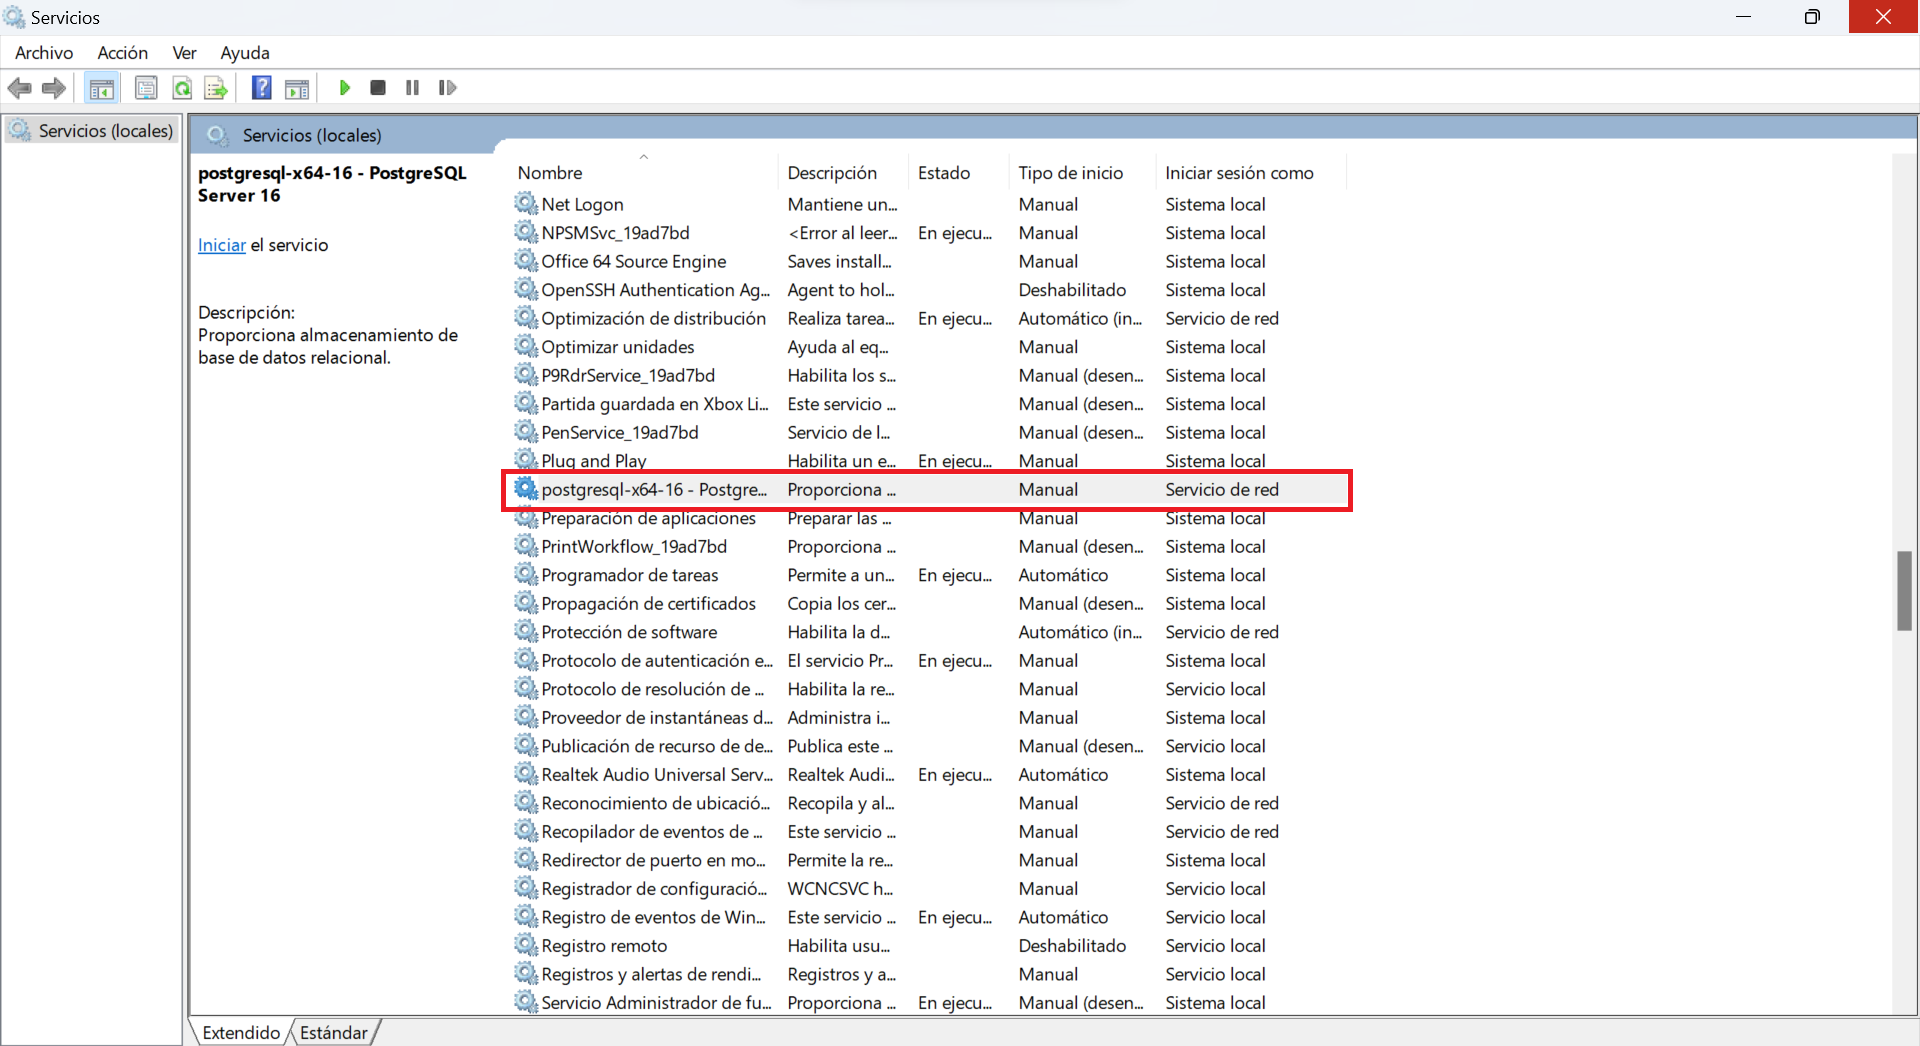
\includegraphics[width=0.90\textwidth]{figures/serviciosConfig.png}
     \caption{Captura de pantalla de la aplicación de servicios.}
    \label{fig:serviciosConfig}
    \end{figure}

    \item El último paso consiste en registrar el servidor a través del administrador de base de datos instalado en el equipo, en este caso pgAdmin. 
    
    Una vez que tengamos libre el puerto 5432, podemos registrar un nuevo servidor en dicho puerto que acceda a la base de datos de Broadsea. Para ello abrimos el administrador de la base de datos PostgreSQL, pgAdmin 4, y registramos un nuevo servidor. Los parámetros de configuración de este nuevo servidor se describen en el \textit{docker-compose.yml} y en la sección 3 del archivo \textit{.env}. Los parámetros fundamentales son:

    \begin{lstlisting}[language=sh]
        host = 127.0.0.1
        port = 5432
        user = postgres
        password = mypass\end{lstlisting}
    
    \item Tras registrar el servidor correctamente, debe aparecer una base de datos con cinco esquemas: \code{demo\_cdm}, \code{demo\_cdm\_results}, \code{public}, \code{webapi}, \code{webapi\_security}. Para comprobar que se ha establecido una conexión correcta con la base de datos, sin pérdida de información, se puede comprobar el número de filas que recupera pgAdmin de la tabla \code{person} del esquema \code{demo\_cdm}, tal y como se muestra en la Figura \ref{fig:pgAdmin}.

    \begin{figure}[H]
    \centering
    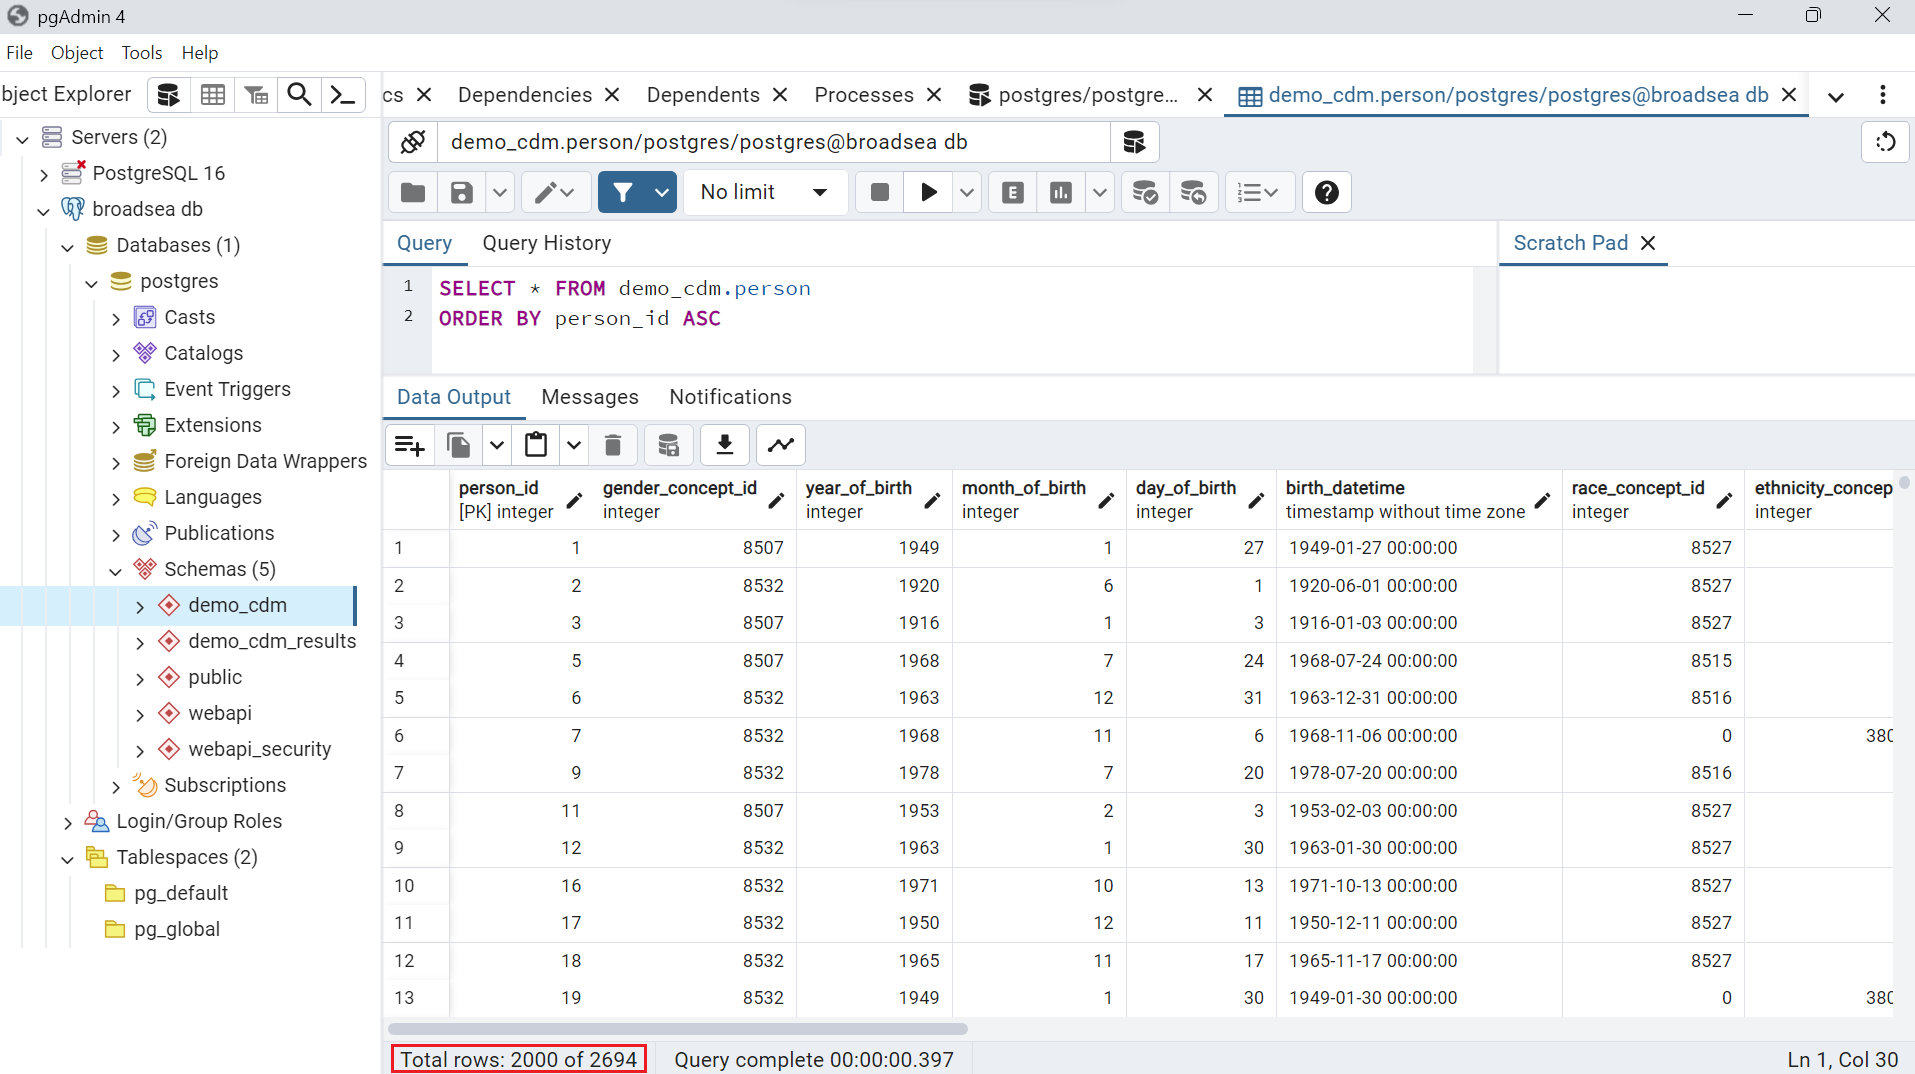
\includegraphics[width=0.90\textwidth]{figures/pgAdmin.png}
     \caption{Captura de pantalla de pgAdmin.}
    \label{fig:pgAdmin}
    \end{figure}

    El número de filas que recupere pgAdmin debe ser igual al número de personas que muestra ATLAS en la sección Data Sorce/Dashboard, en este caso son 2694 personas (Figura \ref{fig:dashboardEJ}).

    \begin{figure}[H]
    \centering
    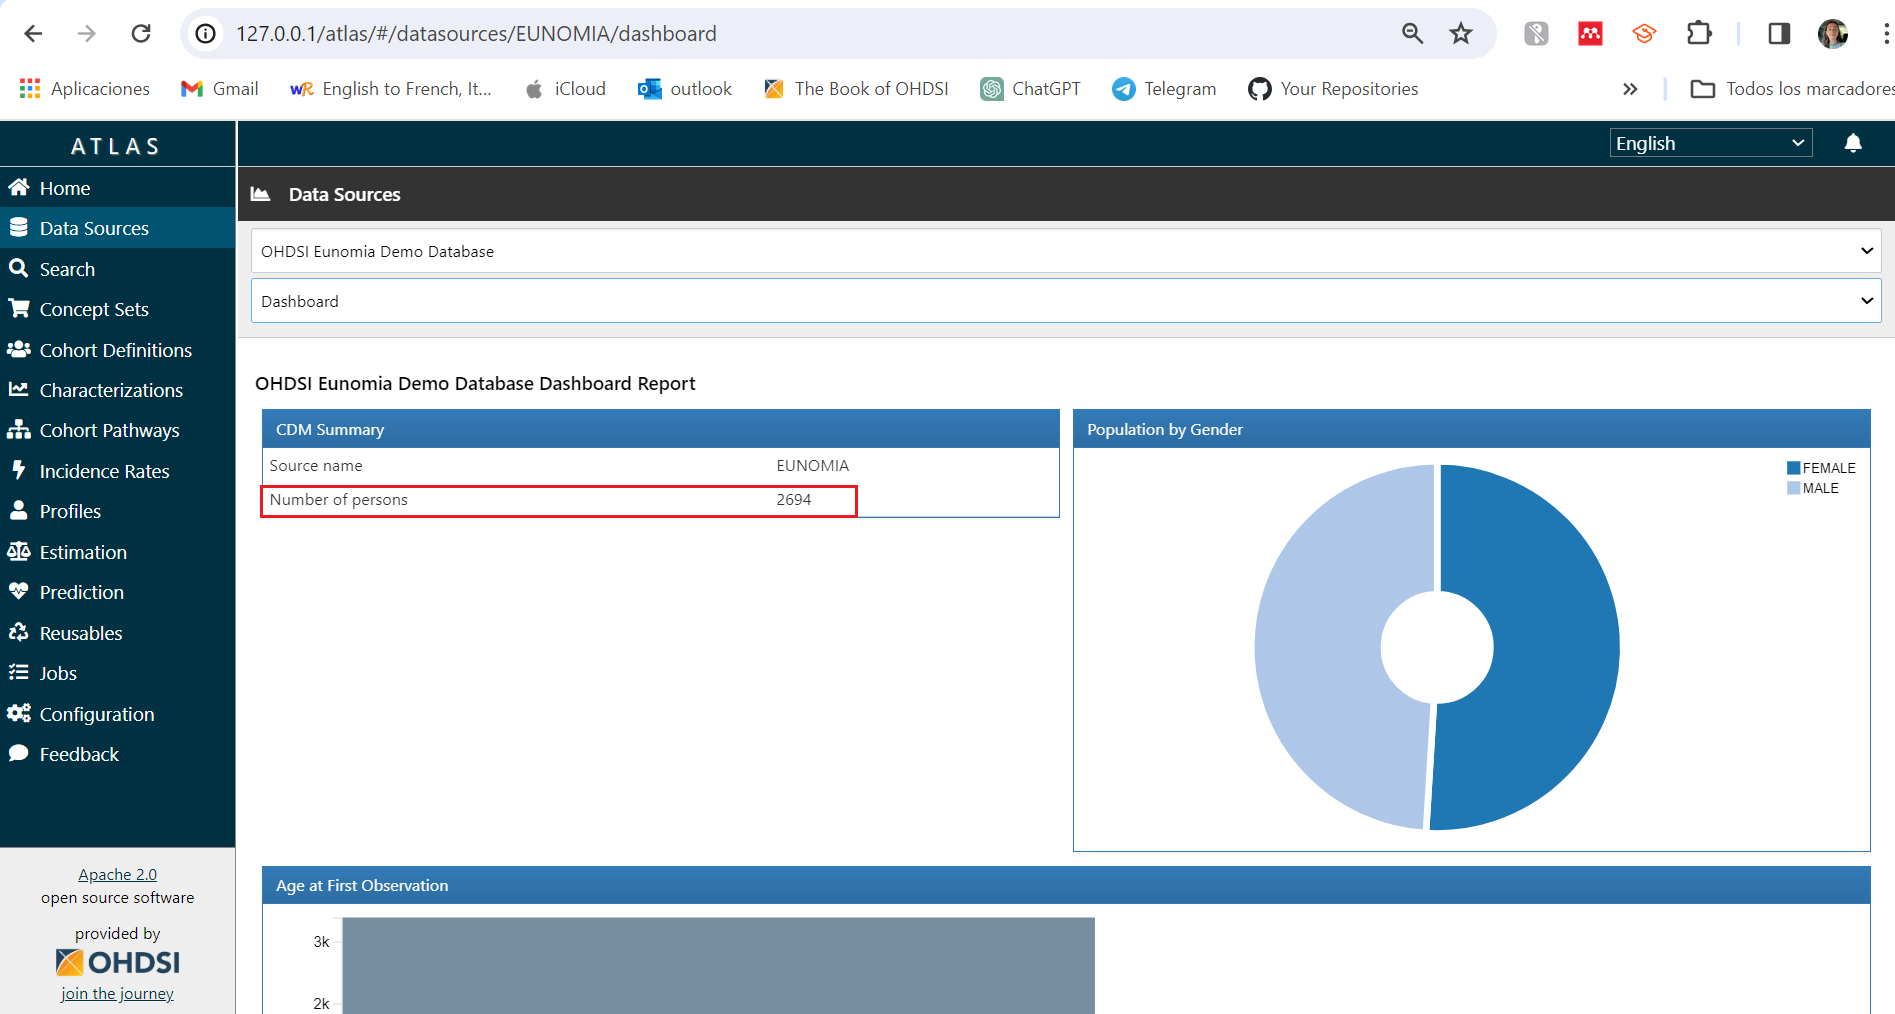
\includegraphics[width=0.90\textwidth]{figures/dashboardEJ.png}
     \caption{Captura de pantalla de ATLAS Data Sources/Dashboard.}
    \label{fig:dashboardEJ}
    \end{figure}

    \item Por último, otra forma de comprobar que la conexión es correcta y una forma alternativa de realizarla, con el fin de detectar posibles problemas durante la implementación, es ejecutar el siguiente script de código en R, que realiza la conexión con la base de datos a través de RStudio:

    \begin{figure}[H]
    \centering
    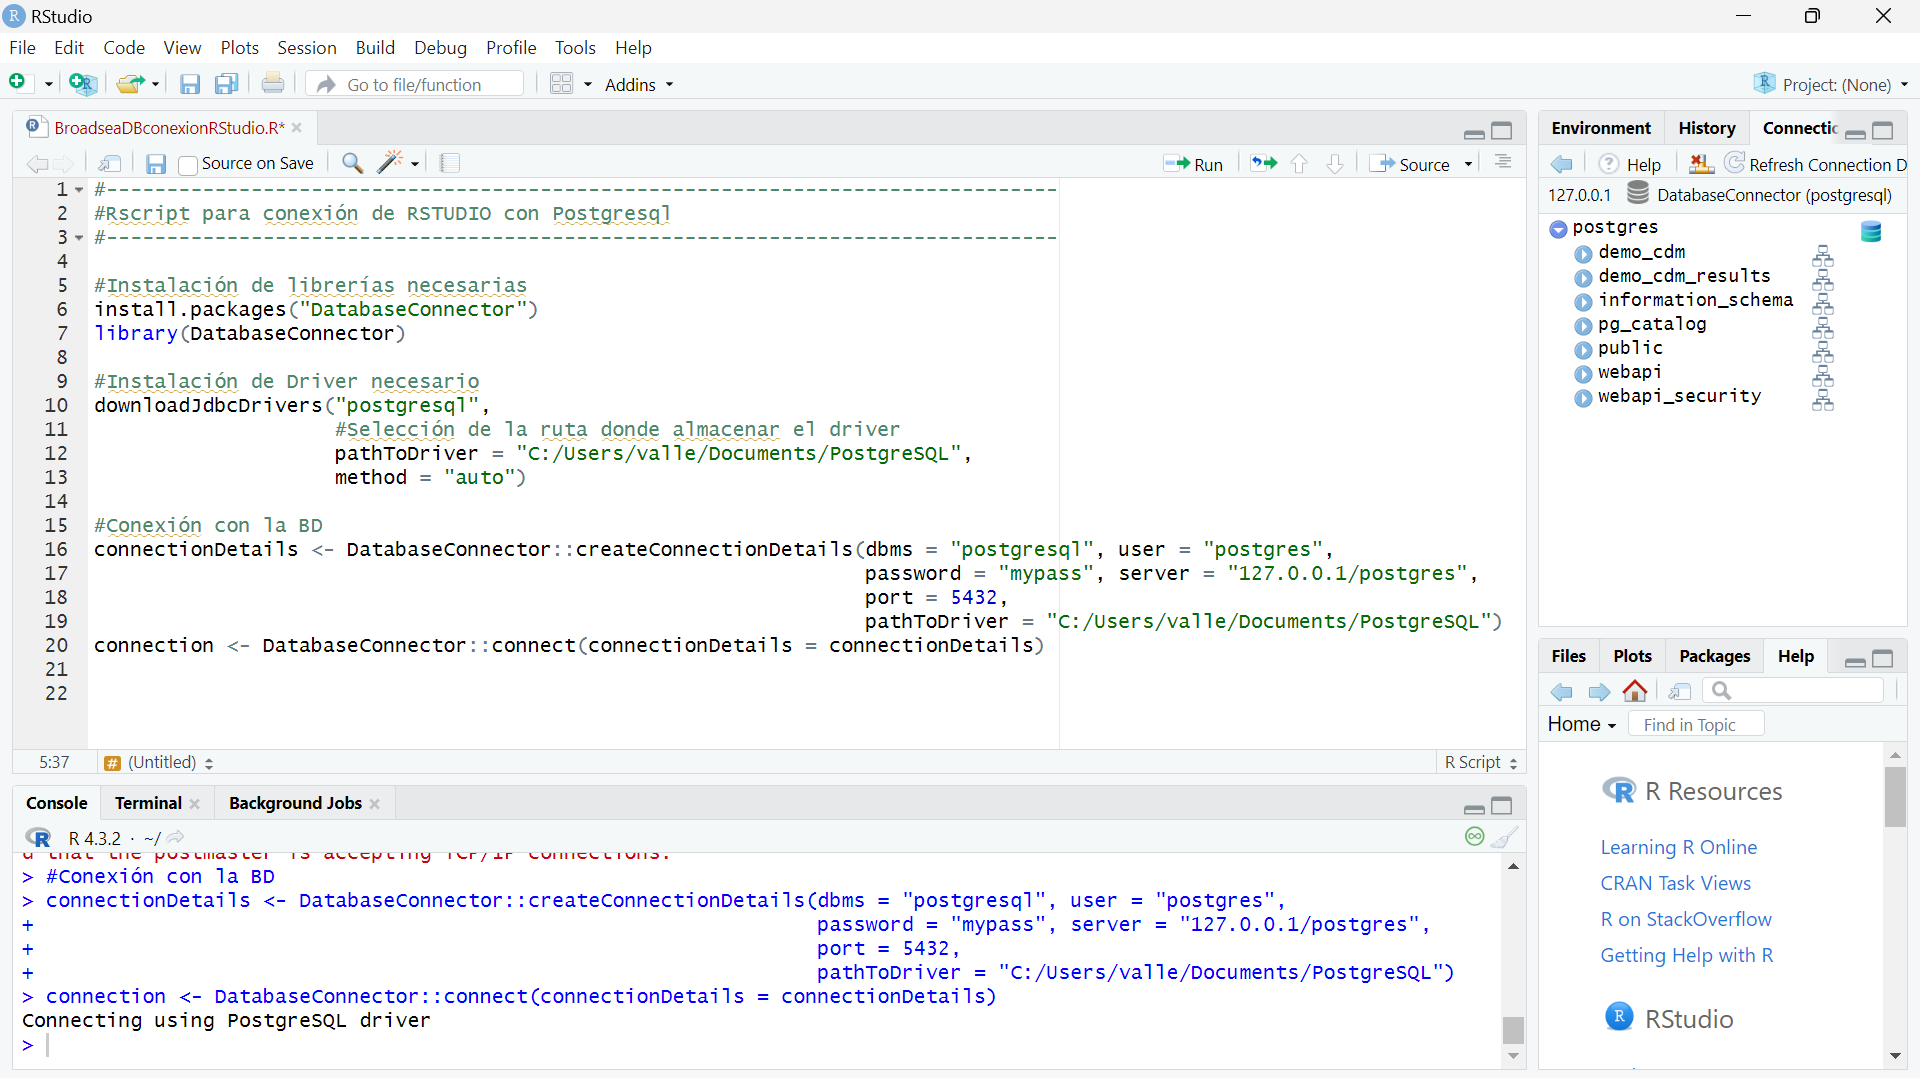
\includegraphics[width=0.90\textwidth]{figures/RStudio.png}
     \caption{Captura de pantalla de script de RStudio.}
    \label{fig:RStudio}
    \end{figure}
    
\end{enumerate}

\section{Solución de posibles problemas}

\subsubsection{Error: Connection timeout expired}
Al entrar en la base de datos de Eunomia e introducir la contraseña aparece el error.

    \begin{figure}[H]
    \centering
    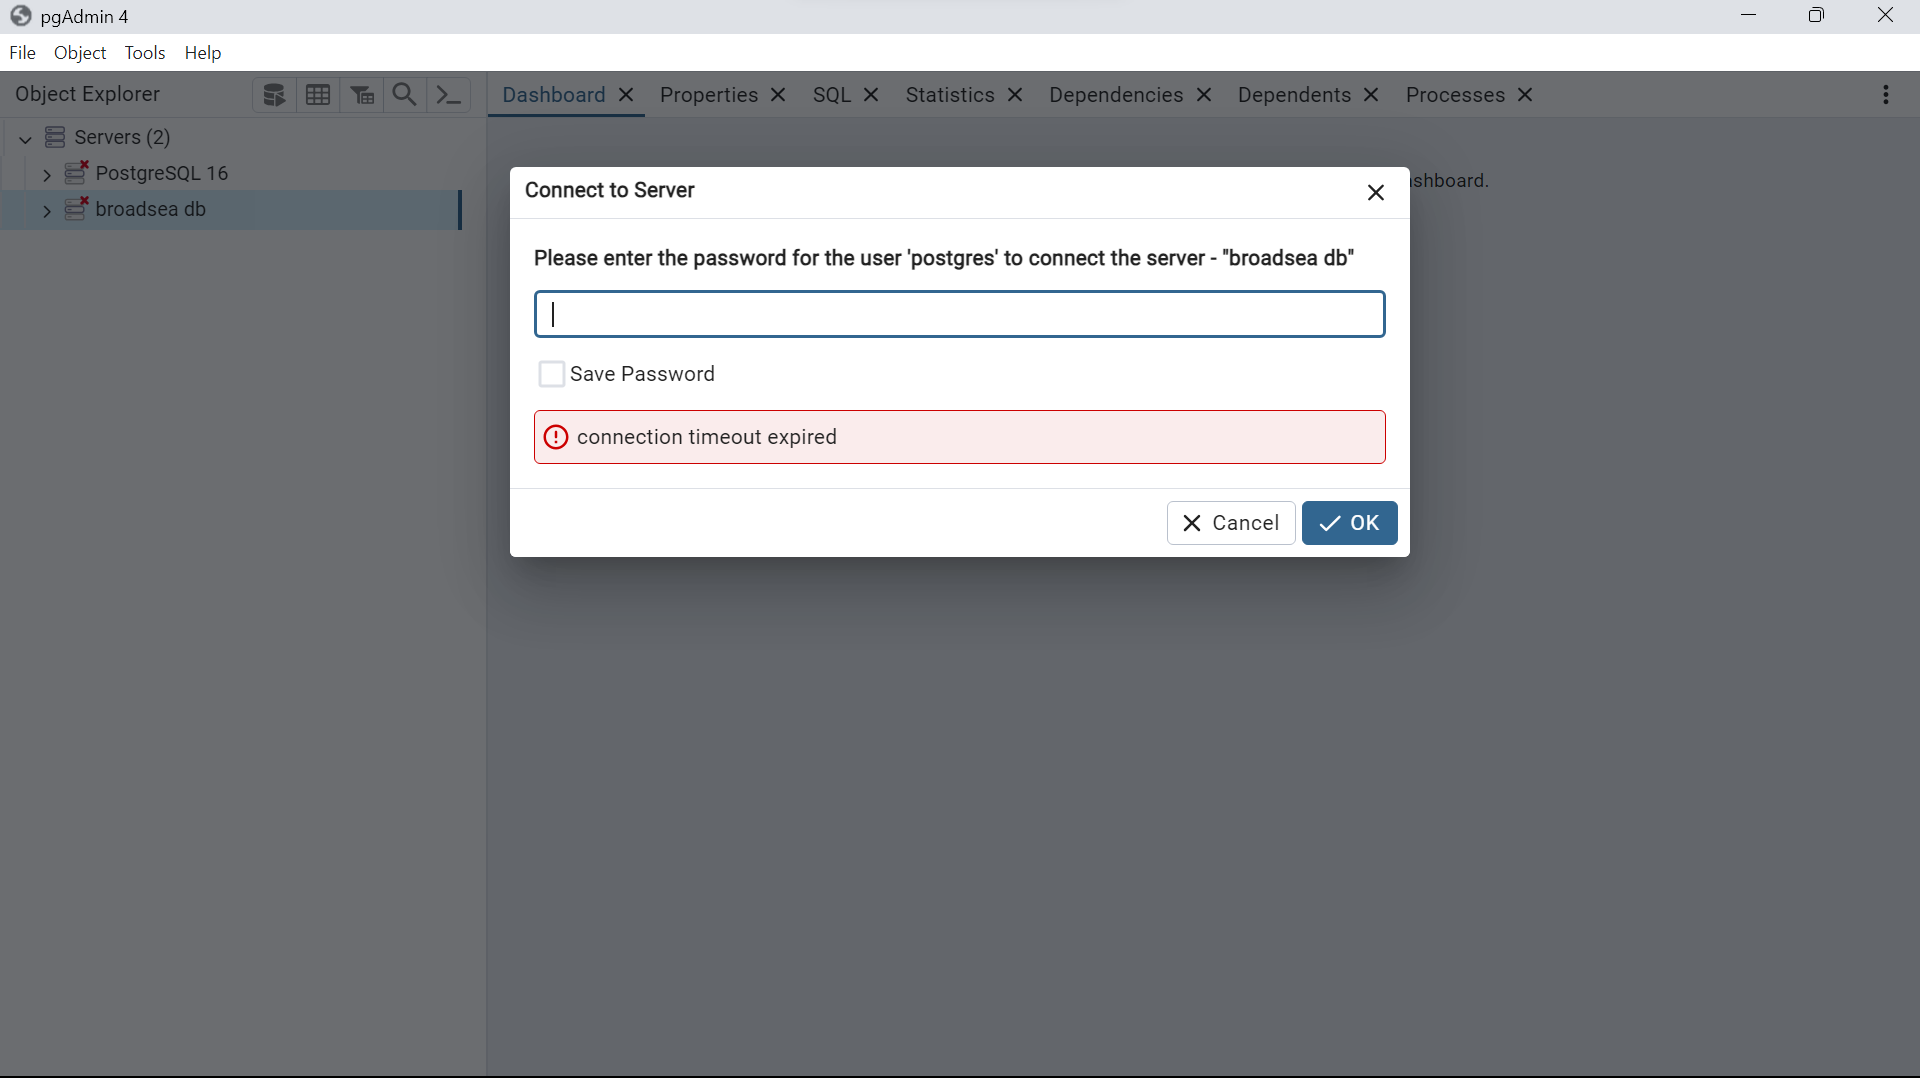
\includegraphics[width=0.90\textwidth]{figures/Error03ConnTime.png}
     \caption{Captura de pantalla de error.}
    \label{fig:Error03ConnTime}
    \end{figure}

Solución: Enciende el contenedor de docker.

\subsubsection{No permite establecer la conexión por puerto ocupado.}

 
    \chapter{Conexión local con otras BD}

\section{Obtener otras BD}

- synthea
- synpuf


\section{Establecer la conexión}

- Mediante SQL queries
- Activando la seguridad
    \chapter{Configuración del Vocabulario}

El vocabulario no viene enteramente configurado en ATLAS Broadsea sino tan solo una pequeña demo adjunta a la base de datos de Eunomia, tal y como se describe en el repositorio de github de la \href{https://github.com/OHDSI/Broadsea-Atlasdb/tree/main}{ Base de datos de Broadsea}.

Por tanto, para poder utilizar ATLAS en profundidad se requiere la instalación y configuración del Vocabulario más extenso. OHDSI propone, en el repositorio de github de \href{https://github.com/OHDSI/Broadsea}{Broadsea} dos formas de configurar el vocabulario de Broadsea: (1) de forma manual (2) a través de Apache Solr. 

\section{Configuración manual}

La configuración manual del vocabulario requiere descargrar el vocabulario directamente desde ATHENA, instalarlo manualmente en el directorio local de Broadsea y ejecutar el contenedor docker encargado de montar el vocabulario en Broadsea. 


\subsection{Requisitos previos}

Para configurar el vocabulario manualmente,  se debe haber descargado el vocabulario y configurado el directorio local de Broadsea. Este procedimiento se ha seguido gracias a los foros \href{https://forums.ohdsi.org/t/downloading-omop-cdm-version-5-vocabulary-data/3321/3}{Downloading OMOP cdm version 5 vocabulary data} y \href{https://forums.ohdsi.org/t/march-to-the-broadsea/20576}{March to the Broadsea} y el tutorial de yotutube \href{https://www.youtube.com/watch?v=FCHxAQOBptE}{Demo: Getting Vocabularies Into My OMOP CDM}.

\begin{enumerate}

    \item Descargar el vocabulario desde la herramienta online de  \href{https://athena.ohdsi.org/}{ATHENA}.Para ello, acceder al menú de descarga \code{Download}. En este momento se presenta un listado de todos los vocabularios que contiene ATHENA entre los que algunos aparecen preseleccionados. Cada usuario puede seleccionar o deseleccionar los vocabularios que le interesen para el estudio que esté realizando. En este caso, se descargará el vocabulario que ATHENA sugiere por defecto.
    
    \begin{figure}[H]
        \centering
        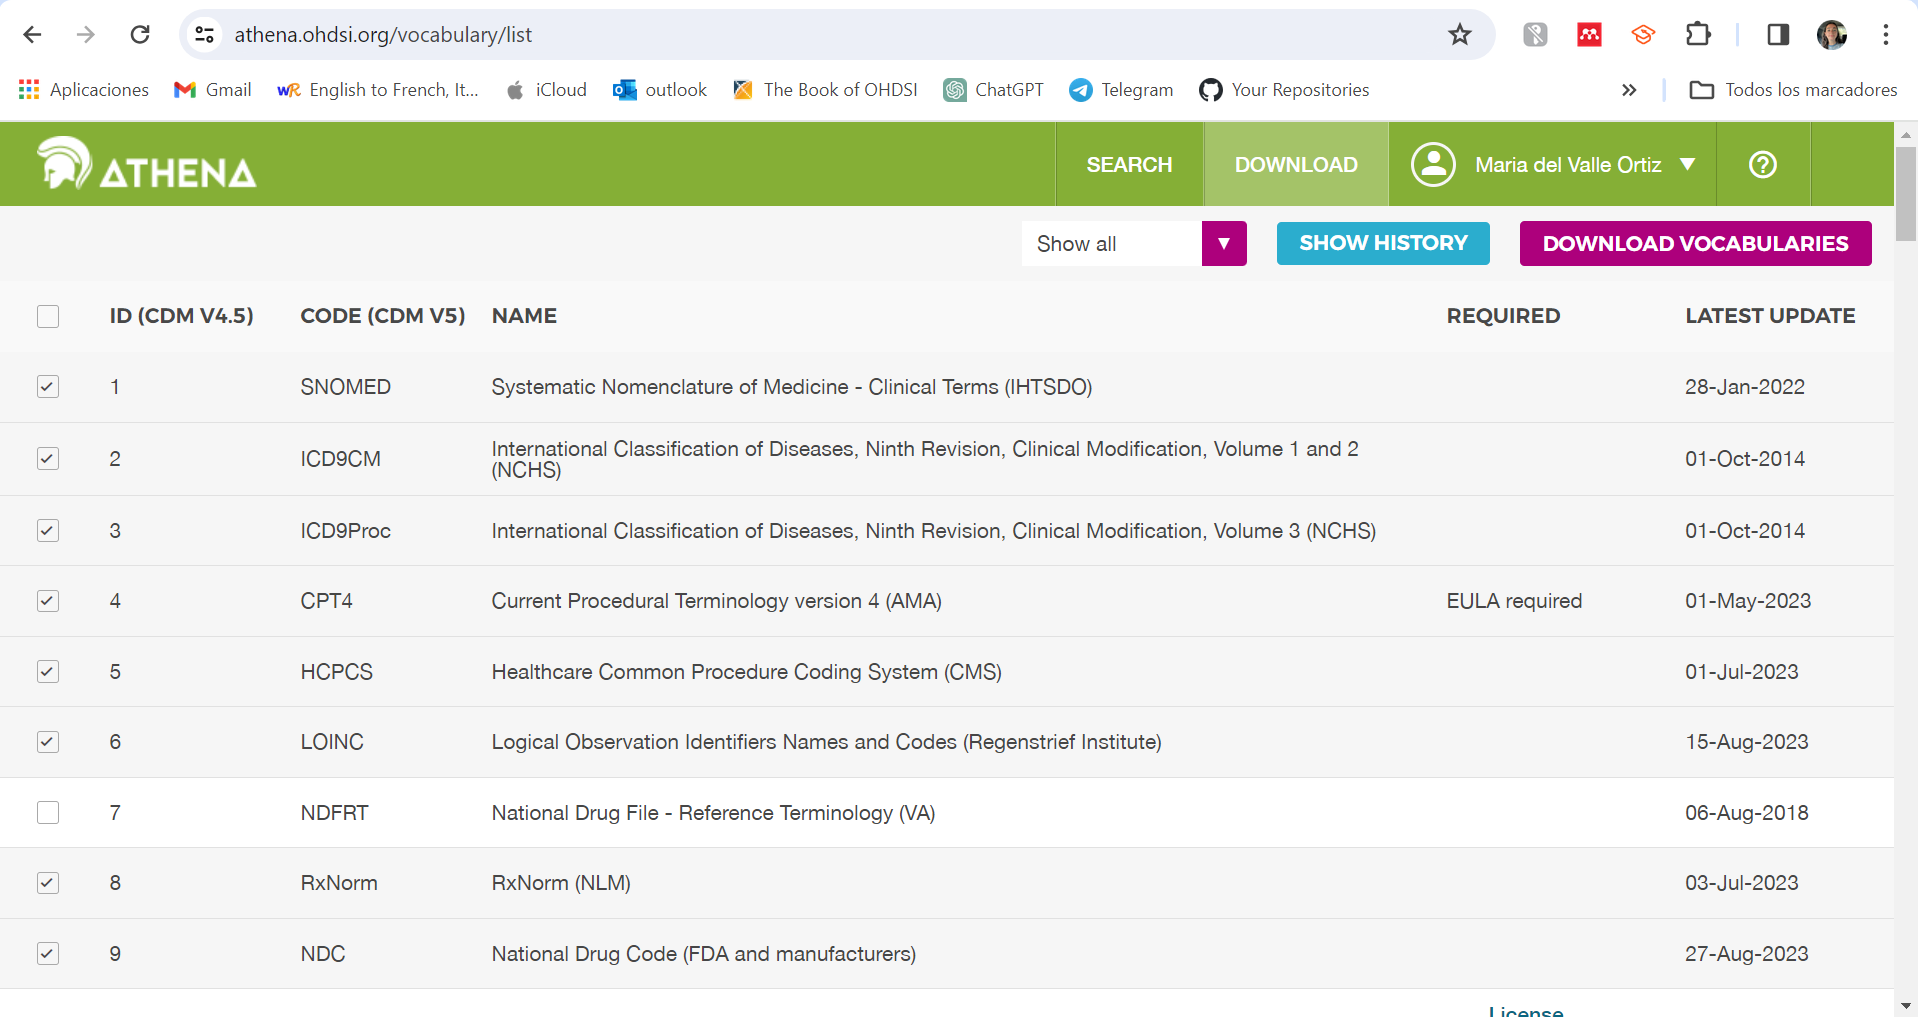
\includegraphics[width=0.90\textwidth]{figures/athenaPreDownload.png}
        \caption{Captura de pantalla de la preselección de vocabularios para descargar.}
        \label{fig:athenaPreDownload}
    \end{figure}

    \item La descarga requiere registrar un usuario con un correo electrónico válido al que se enviará un link personal que permitirá la descarga de un archivo .zip con el vocabulario seleccionado. También desde ATHENA en la pestaña \code{SHOW HISTORY} muestra el estado en el que se encuentra la descarga del vocabulario y, una vez que esté listo, permite la descarga directa del zip.

    \item El archivo zip que se descarga, una vez descomprimido, muestra varios archivos .csv con las tablas que conforman el Vocabulario y otros archivos CPT4 que requieren de una configuración adicional. En este caso, no se utilizará el vocabulario de CPT4 por lo que no se realizará esta configuración, sin embargo, viene bien explicada en el tutorial de youtube adjunto al principio de la sección.

      \begin{figure}[H]
        \centering
        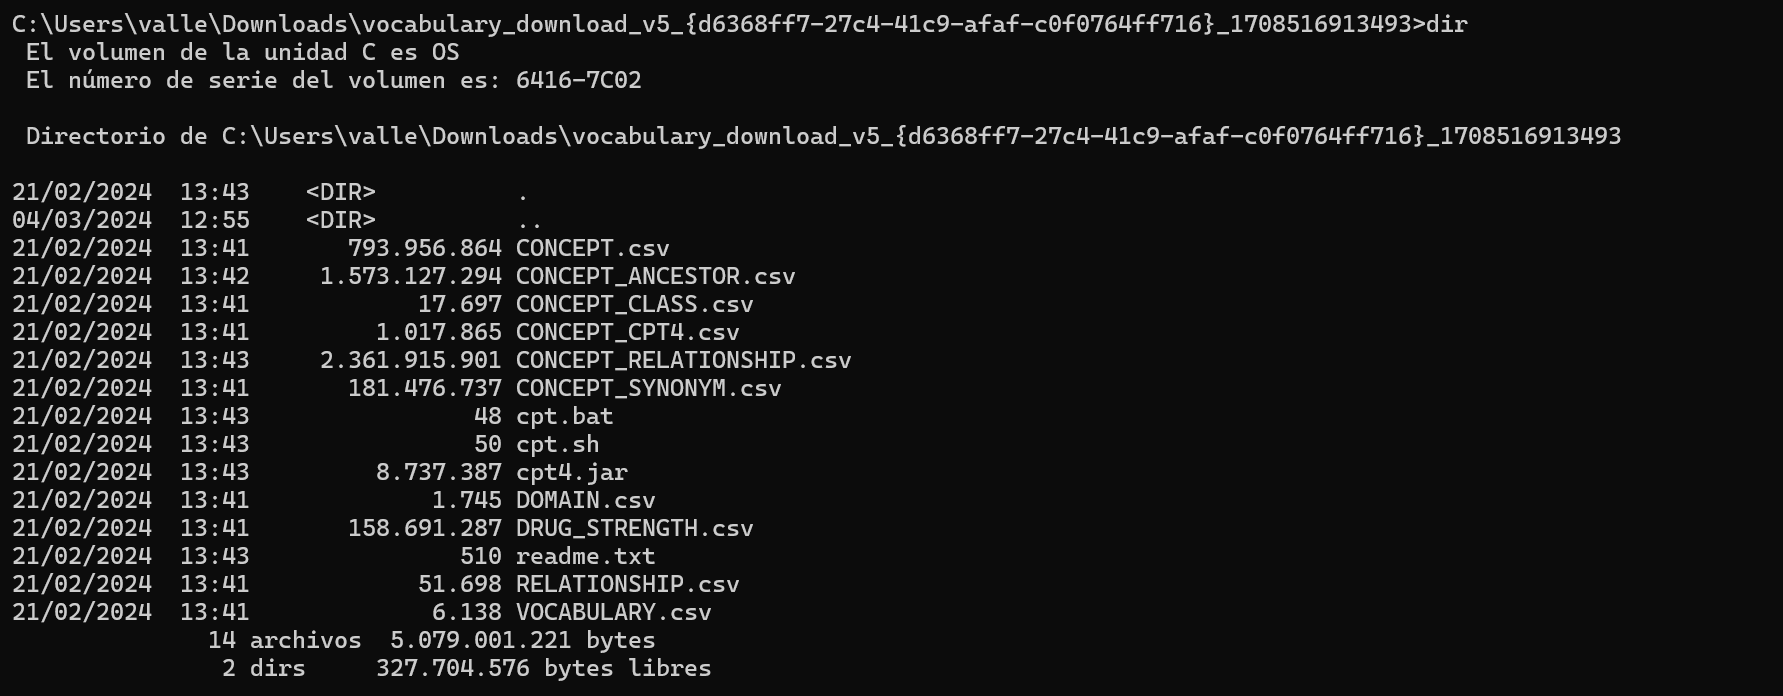
\includegraphics[width=0.90\textwidth]{figures/vocabDownload.png}
        \caption{Captura de pantalla de archivos descargados del vocabulario.}
        \label{fig:vocabDownload}
    \end{figure}

    \item Por último, los archivos descargados del vocabulario deben almacenarse en el directorio local de Broadsea, concretamente en la ruta \code{Broadsea/omop\_vocab/files}. En caso de no existir la carpeta \code{/files}, crearla manualmente. Este paso es muy importante.

\end{enumerate}

\subsection{Deployment}

Configurar el vocabulario requiere establecer una configuración avanzada del contenedor Docker de Broadsea. Si bien, la primera vez que se inicializó el contenedor se ejecutó el perfil \code{default} ahora se va a ejecutar específicamente el perfil \code{omop-vocab-pg-load}. Esta opción se especifica en la sección \href{https://github.com/OHDSI/Broadsea?tab=readme-ov-file#omop-vocab-loading}{OMOP Vocab Loading} del repositorio de Broadsea. También ha sido de utilidad el repositorio \href{https://github.com/OHDSI/WebAPI/wiki/CDM-Configuration}{CDM Configuration} y el mismo forum \href{https://forums.ohdsi.org/t/march-to-the-broadsea/20576}{March to the Broadsea}.

Para acceder a la información y configuración avanzada del perfil se puede acceder al \code{docker-compose.yml} y a la sección 9 del archivo \code{.env}, aunque este caso no será necesario realizar ninguna modificación sobre los mismos.

\begin{enumerate}

    \item Para comenzar la configuración del vocabulario es necesario inicializar el contenedor \code{omop-vocab-load}. Ejecutar la siguiente línea de código en el \code{cmd}:

    \begin{lstlisting}[language=sh]
    docker compose --profile omop-vocab-pg-load up -d\end{lstlisting}

    Este comando da lugar el siguiente resultado.

      \begin{figure}[H]
        \centering
        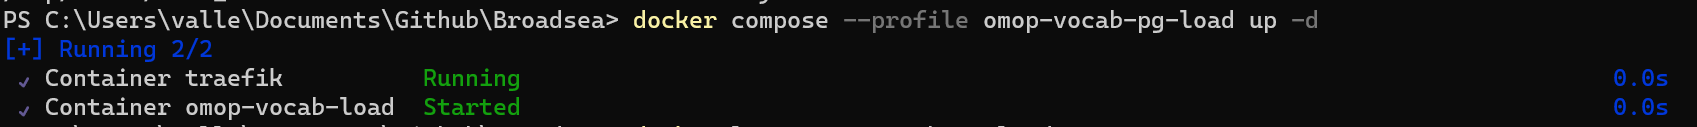
\includegraphics[width=0.90\textwidth]{figures/composeProfVocabLoad.png}
        \caption{Captura de pantalla de comando para iniciar el perfil docker.}
        \label{fig:composeProfVocabLoad}
    \end{figure}

    \item A partir de este momento comienza la instalación del perfil, por lo que es muy importante tener abierto el \code{logs} de Docker para poder observar que el proceso se realiza correctamente. El proceso puede durar unas horas y una vez que se finaliza, el log muestra un mensaje que advierte que el contenedor puede ser eliminado y el estado del contenedor pasa a ser ''Exited''. El resultado es la creación de un nuevo esquema en la base de datos llamado ''omop\_vocab'' con todos los archivos descargados del vocabulario. 

    \item El último paso de la configuración es integrar este nuevo esquema a la WebAPI de Broadsea. Este último paso se puede realizar fácilmente de forma manual a través de pgAdmin, abriendo la tabla \code{source\_daimon} del esquema \code{webapi} de la bd de Broadsea.

    La instalación por defecto de Broadsea adjudica la fuente del vocabulario (\code{daimon\_type=1}) al \code{demo\_cdm}, sin embargo, se debe modificar para que apunte al nuevo esquema \code{omop\_vocab} que se ha instalado. Esta modificación se puede realizar directamente haciendo click ssobre la tabla que devuelve la siguiente consulta.

    \begin{lstlisting}[language=sql]
    SELECT * FROM webapi.source_daimon
    ORDER BY source_daimon_id ASC \end{lstlisting}

    El resultado final debe ser similar a la siguiente figura.

    \begin{figure}[H]
        \centering
        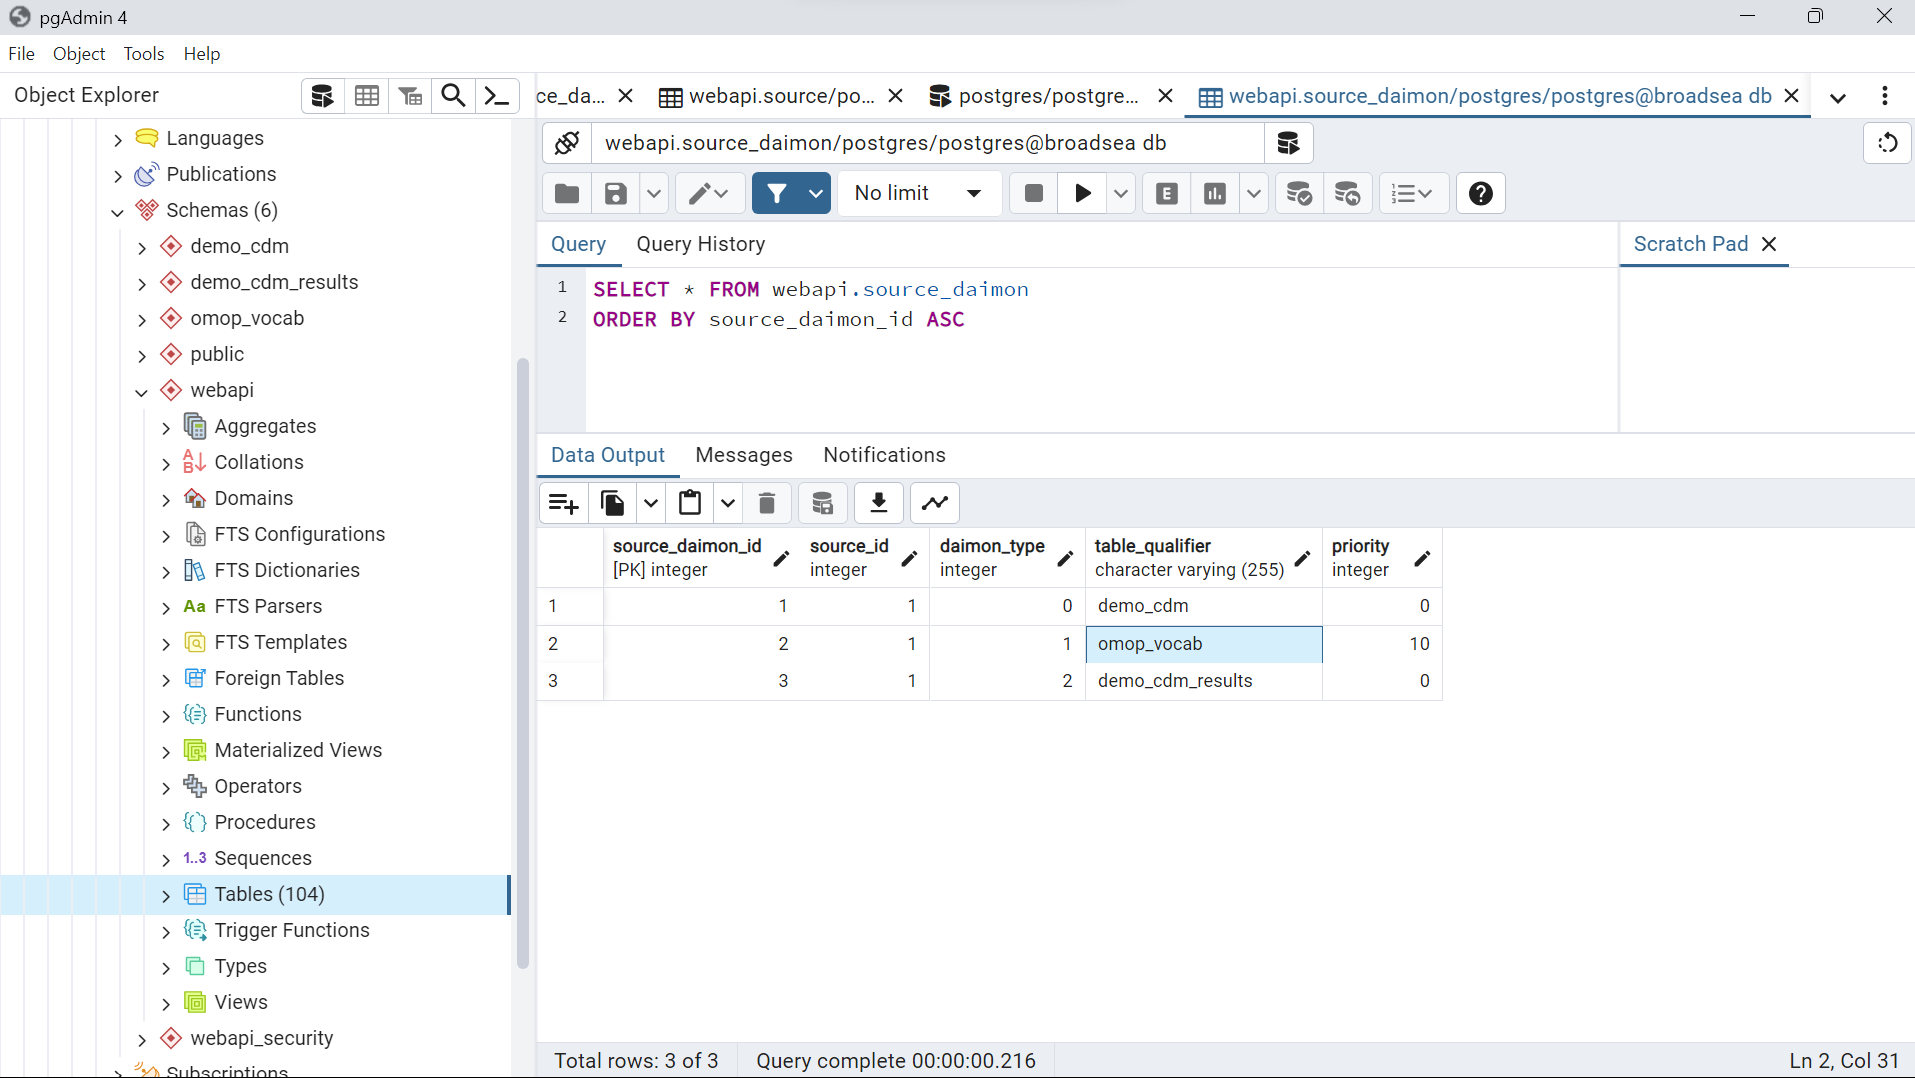
\includegraphics[width=0.90\textwidth]{figures/omopVocabResult.png}
        \caption{Captura de pantalla de la integración final del vocabulario descargado con la webapi}
        \label{fig:omopVocabResult}
    \end{figure}

\end{enumerate}

\subsection{Comprobación de configuración correcta}

Para comprobar que se ha configurado correctamente el vocabulario en la base de datos de Broadsea, se puede consultar el administrador de la base de datos o realizar directamente una búsqueda en ATLAS.

\begin{enumerate}

    \item En primer lugar, desde el administrador de la base de datos, pgAdmin, se debe comprobar que el vocabulario se ha instalado correctamente y no se han instalado tablas vacías. Para ello basta con seleccionar cualquier tabla del esquema \code{omop\_vocab} y mostrar todas las filas. Las tablas más significativas son la tabla \code{vocabulary}, que muestra todos los vocabularios que se han insertado, y la tabla \code{concept} que reúne todos los conceptos definidos en cada vocabulario. Para esta implementación la primera tabla muestra un total de 59 filas y la segunda, 5.975.392 filas.

    \item En segundo lugar, se puede comprobar que la integración del nuevo esquema con el vocabulario haya sido exitosa realizando una búsqueda en el vocabulario directamente desde ATLAS Broadsea. 
    
    El vocabulario demo que venía incluido con Eunomia presentaba muy pocos conceptos por lo que muchas búsquedas de conceptos no devolvían resultado o devolvían muy pocos. Para este manual, se comprobó que antes de realizar la configuración del vocabulario, al buscar ''diabetes'' solo se obtenía un resultado, como se muestra en la figura \ref{fig:ejDiabetesVacio}. Sin embargo, después de configurar correctamente, se obtienen hasta 20602 resultados, como muestra la figura \ref{fig:ejDiabetsFull}.

        \begin{figure}[H]
        \centering
        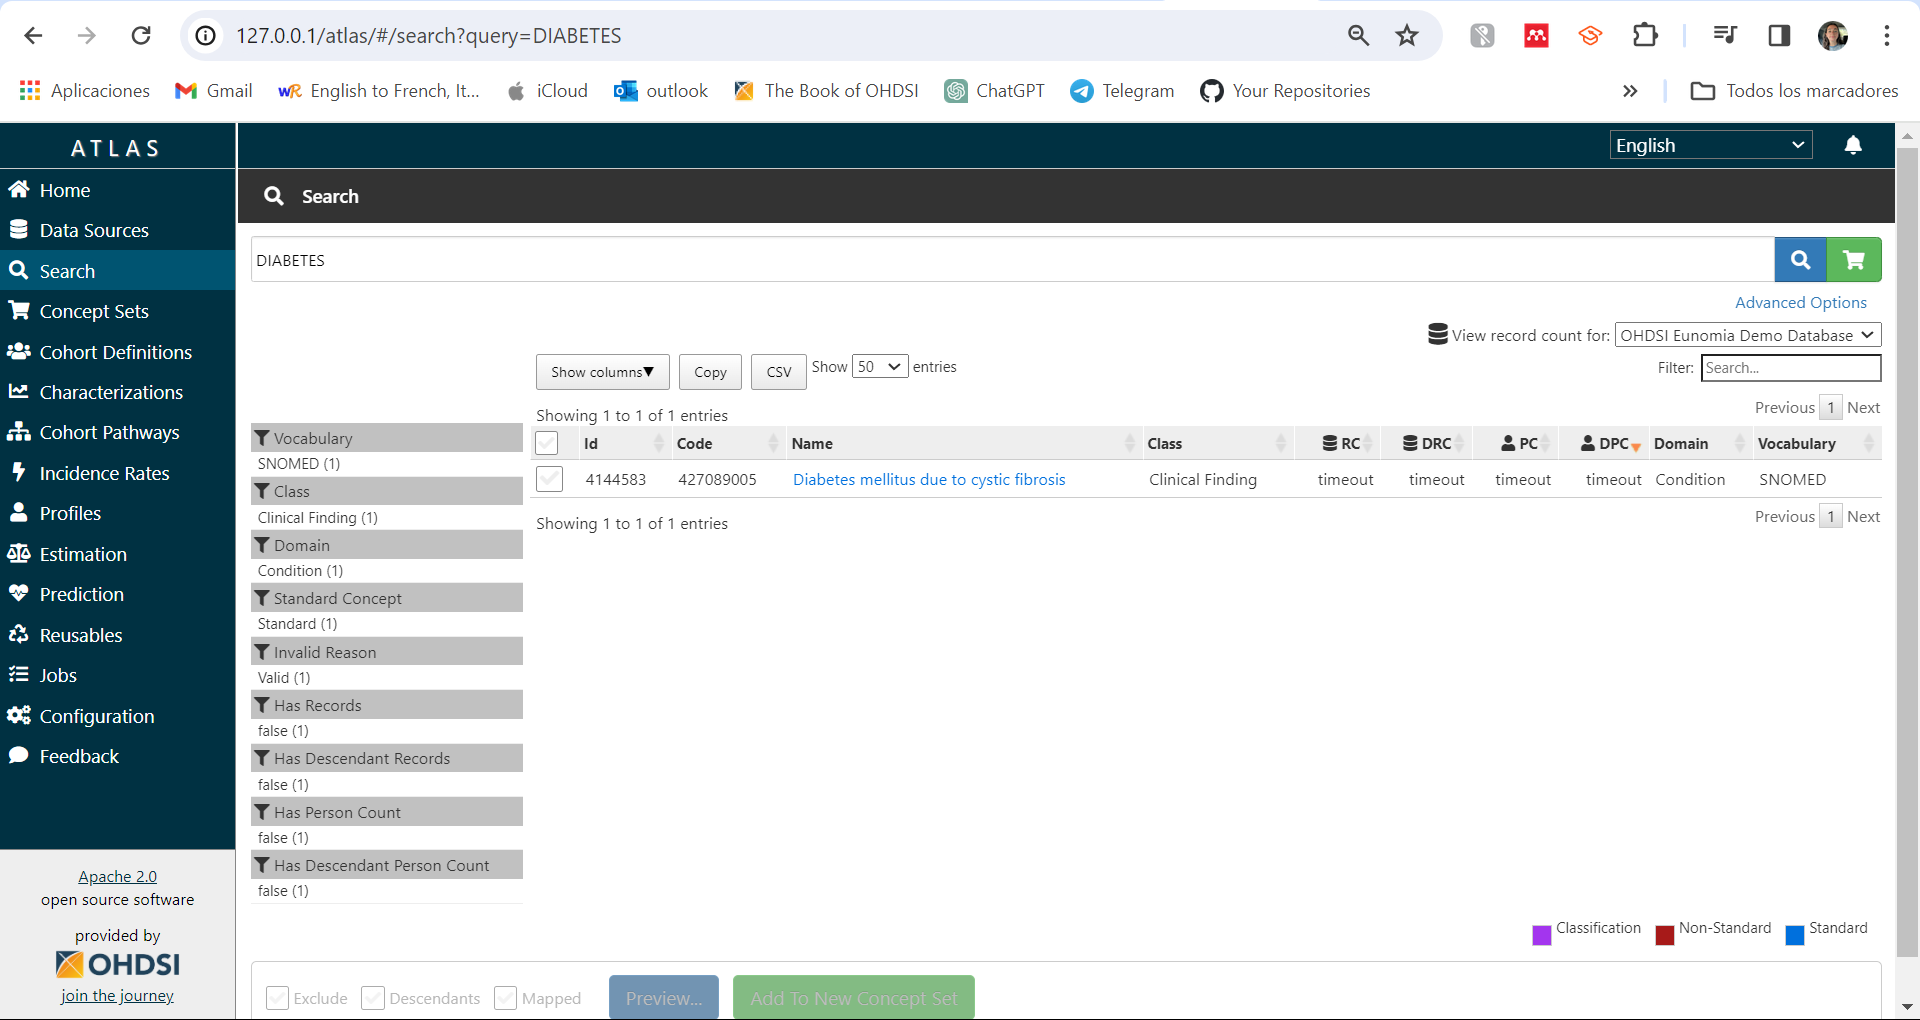
\includegraphics[width=0.90\textwidth]{figures/ejDiabetesVacio.png}
        \caption{Captura de pantalla de la búsqueda en el vocabulario antes de la configuración}
        \label{fig:ejDiabetesVacio}
    \end{figure}

      \begin{figure}[H]
        \centering
        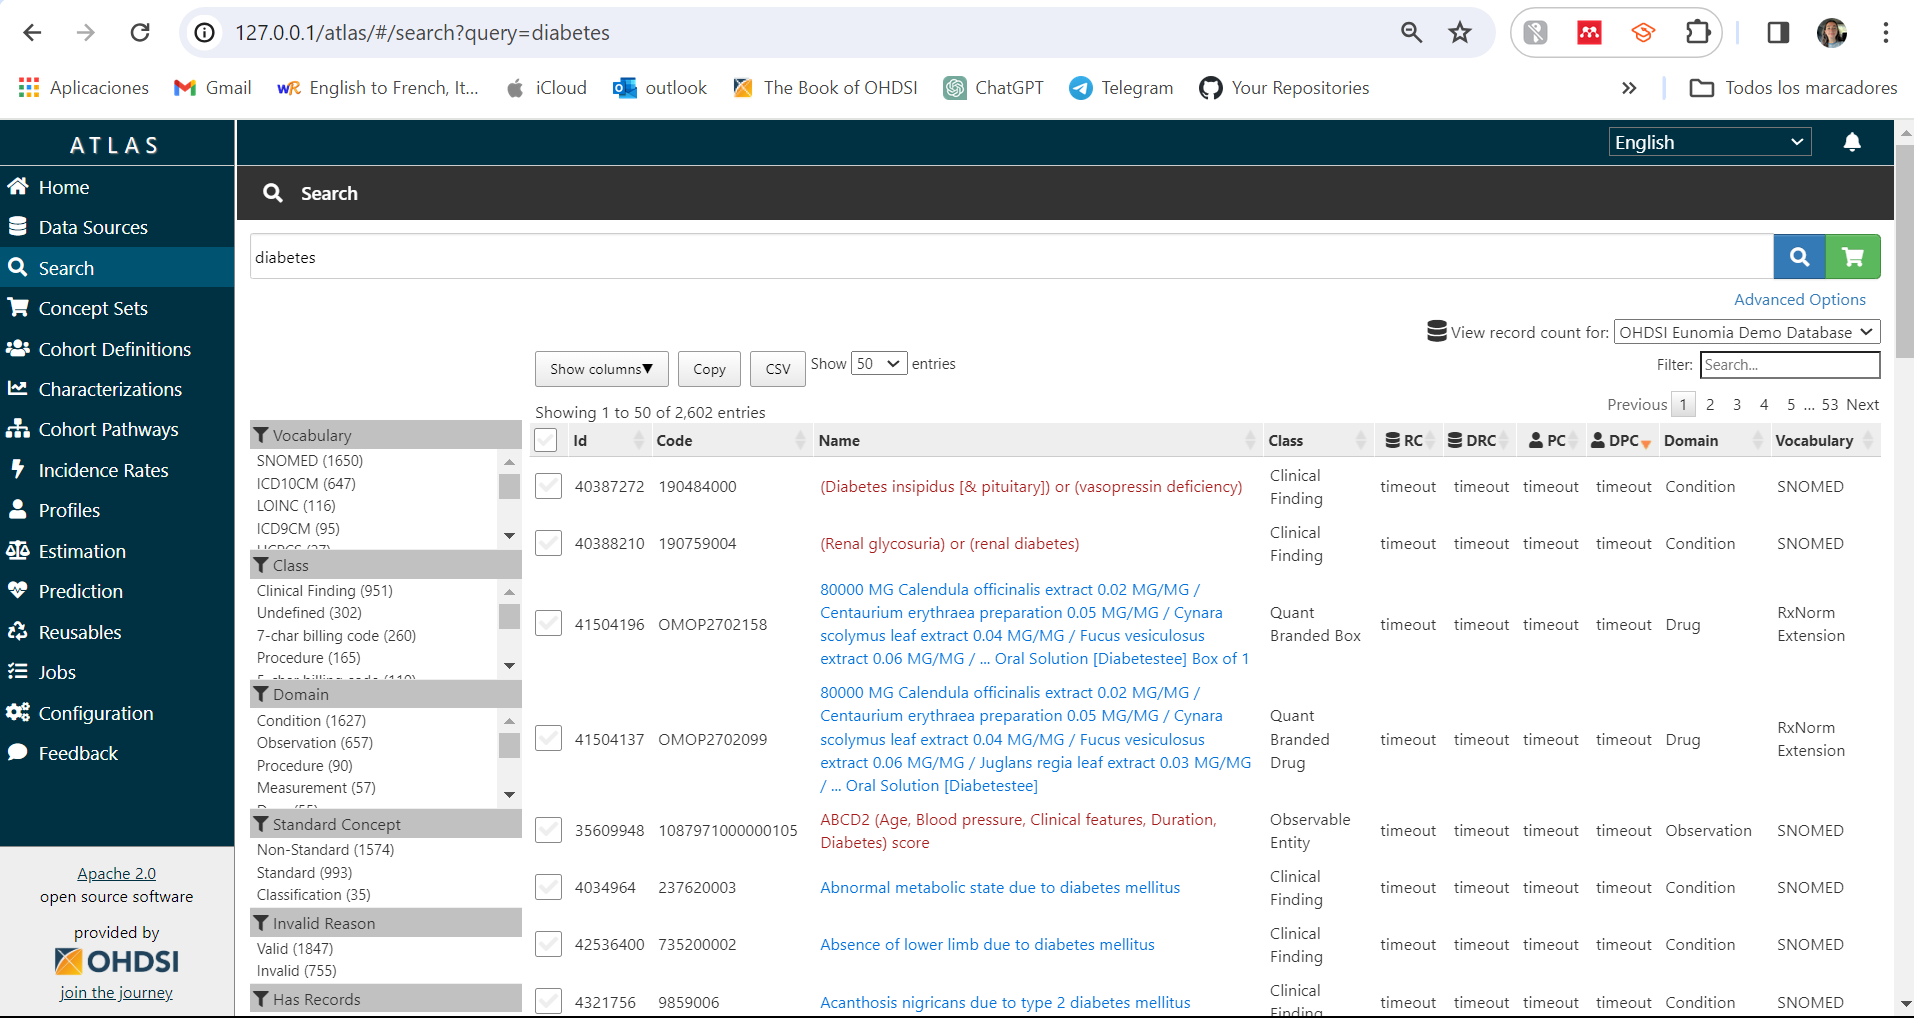
\includegraphics[width=0.90\textwidth]{figures/ejDiabetsFull.png}
        \caption{Captura de pantalla de la búsqueda en el vocabulario después de la configuración}
        \label{fig:ejDiabetsFull}
    \end{figure}

    \item Por último, se puede realizar una comprobación extra accediendo a la dirección \code{http://127.0.0.1/WebAPI/source/refresh} en el navegador, que imprime en pantalla las fuentes que se están utilizando en la configuración de Broadsea. El resultado debe ser similar al siguiente, prestando especial atención a que aparezca \code{omop\_vocab} como fuente del vocabulario:


    \begin{lstlisting}[language=html]
    [{"sourceId":1,"sourceName":"OHDSI Eunomia Demo Database","sourceDialect":"postgresql","sourceKey":"EUNOMIA","daimons":[{"sourceDaimonId":1,"daimonType":"CDM","tableQualifier":"demo_cdm","priority":0},{"sourceDaimonId":3,"daimonType":"Results","tableQualifier":"demo_cdm_results","priority":0},{"sourceDaimonId":2,"daimonType":"Vocabulary","tableQualifier":"omop_vocab","priority":10}]}] \end{lstlisting}

    
\end{enumerate}


\subsection{Solución de posibles errores}

\subsubsection{Error: can't cd to /temp/files: No such files or directory}

Al inicializar el perfil \code{omop-vocab-load} el contenedor no se construye correctamente y el log muestra el siguiente aviso, tal y como se muestra en la figura.

      \begin{figure}[H]
        \centering
        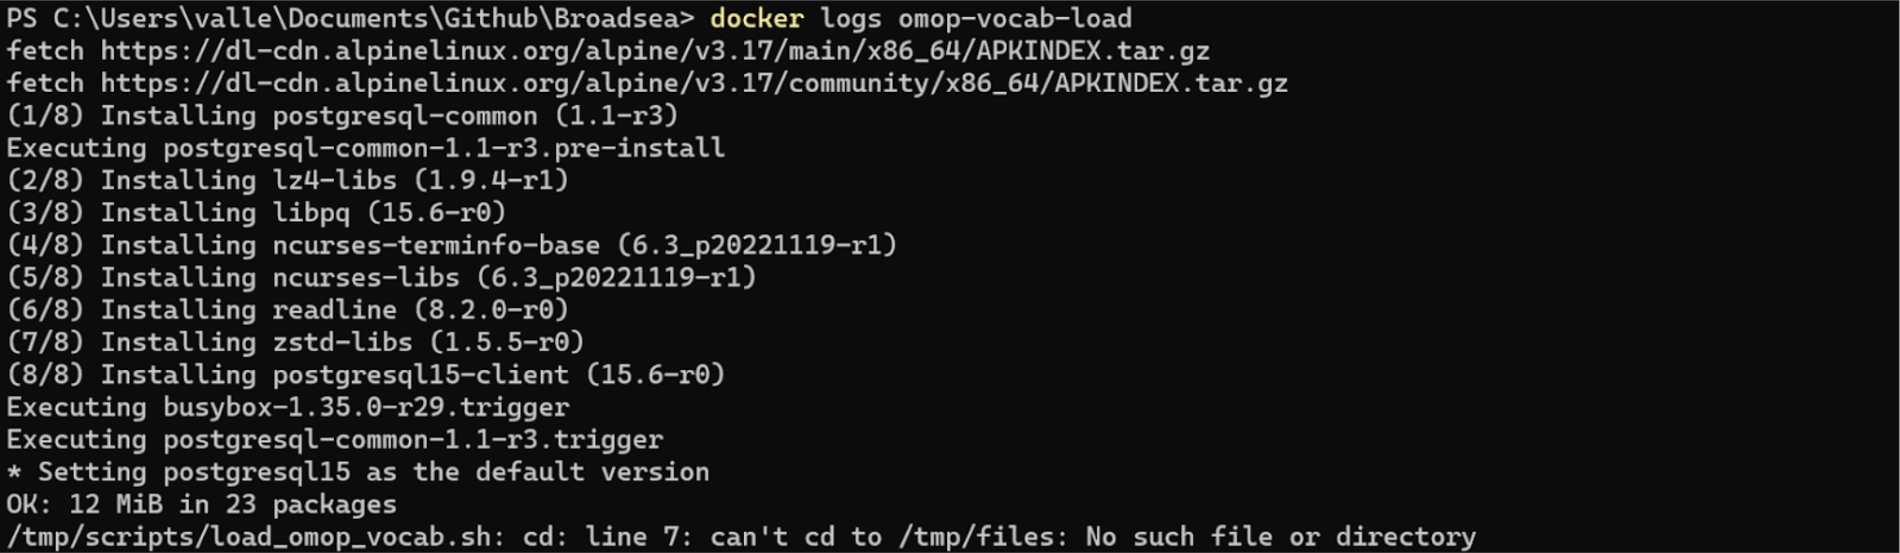
\includegraphics[width=0.90\textwidth]{figures/error05NoFile.png}
        \caption{Captura de pantalla de la búsqueda en el vocabulario después de la configuración}
        \label{fig:error05NoFile}
    \end{figure}
    
Solución: Crear manualmente la carpeta /files

\subsubsection{Error: El contenedor se construye correctamente pero se construye vacío}

Al inicializar el perfil \code{omop-vocab-load} el contenedor se construye en pocos segundos aparentemente correctamente. Incluso es posible que aparezca en el administrador de la base de datos pero aparece el esquema vacío o las tablas del esquema vacías, sin filas.

Solución: La carpeta /files debe contener los archivos .csv que se han descargado de ATHENA.

\section{Otras configuraciones avanzadas}

En este punto el vocabulario ya está perfectamente instalado y configurado, sin embargo, Broadsea ofrece más opciones avanzadas para sacar aún mayor partido de la herramienta. En este manual se presentan dichas opciones aunque no se procederá a su configuración.

\subsection{Configuración de Apache Solr}

ATLAS Broadsea hace uso de Apache Solr a través de diferentes perfiles docker para facilitar la importación del vocabulario y la búsqueda en el mismo. Sin embargo, ambas características aún se encuentras en desarrollo, según la información facilitada en el repositorio de github de \href{https://github.com/OHDSI/Broadsea-Solr}{Broadsea Solr}.

El proceso de configuración de Broadsea Solr se encuentra en aquel mismo repositorio y la descripción de los perfiles que ejecutan los contenedores Solr se presentan en el de \href{https://github.com/OHDSI/Broadsea}{Broadsea}. 

\begin{enumerate}
    \item Con el perfil \code{solr-vocab-with-import} se puede automatizar la importación del vocabulario desde el servidor de Apache en vez de tener que configurarlo manualmente. Sin embargo, esta opción que parece facilitar el trabajo al usuario en la práctica resulta engorrosa, por ello no ha sido cubierta en este manual.
    \item El otro perfil, \code{solr-vocab-no-import} simplemente lanza el servidor Apache ''vacío'' permitiendo la configuración manual del vocabulario desde la GUI de Apache Solr.
\end{enumerate}

Para mayor información o resolución de conflictos consultar los foros de OHDSI o los ''issue'' del repositorio de github.

\subsection{Configuración de PHOEBE}

ATLAS Broadsea puede configurarse junto a PHOEBE, que es una herramienta OHDSI, también disponible \href{https://data.ohdsi.org/PHOEBE/}{online}, que consiste en un recomendador de conceptos del vocabulario, de forma que facilite la construcción de conjuntos de conceptos durante la realización de estudios con ATLAS. 

No existe un repositorio concreto de esta herramienta pero el perfil que implementa el contenedor docker se presenta brevemente en el repositorio de \href{https://github.com/OHDSI/Broadsea}{Broadsea}. También se puede encontrar información relevante en algunos foros de OHDSI como en el de \href{https://forums.ohdsi.org/t/phoebe-2-0/17410}{Phoebe 2.0}.

De igual forma, para mayor información o resolución de conflictos consultar otros foros de OHDSI o los ''issue'' del repositorio de github de Broadsea o ATLAS.

    \bibliographystyle{unsrtnat}
    \bibliography{bibliografia.bib}

        

% Fin del documento
\end{document}
